% !TeX program = pdfLaTeX
\documentclass[12pt]{article}
\usepackage{amsmath}
\usepackage{graphicx,psfrag,epsf}
\usepackage{enumerate}
\usepackage{natbib}
\usepackage{textcomp}
\usepackage[hyphens]{url} % not crucial - just used below for the URL
\usepackage{hyperref}
\providecommand{\tightlist}{%
  \setlength{\itemsep}{0pt}\setlength{\parskip}{0pt}}

%\pdfminorversion=4
% NOTE: To produce blinded version, replace "0" with "1" below.
\newcommand{\blind}{0}

% DON'T change margins - should be 1 inch all around.
\addtolength{\oddsidemargin}{-.5in}%
\addtolength{\evensidemargin}{-.5in}%
\addtolength{\textwidth}{1in}%
\addtolength{\textheight}{1.3in}%
\addtolength{\topmargin}{-.8in}%

%% load any required packages here



\usepackage{amsmath}
\usepackage{amsfonts}
\usepackage{booktabs}
\usepackage{makecell}
\usepackage[usenames, dvipsnames]{color}
\usepackage{multirow}
\usepackage{comment}
\usepackage{booktabs}
\usepackage{longtable}
\usepackage{array}
\usepackage{wrapfig}
\usepackage{float}
\usepackage{colortbl}
\usepackage{pdflscape}
\usepackage{tabu}
\usepackage{threeparttable}
\usepackage{threeparttablex}
\usepackage[normalem]{ulem}
\usepackage{xcolor}
\newcommand{\beginsupplement}{\setcounter{table}{0} \renewcommand{\thetable}{S\arabic{table}}\setcounter{figure}{0} \renewcommand{\thefigure}{S\arabic{figure}}}

\begin{document}


\def\spacingset#1{\renewcommand{\baselinestretch}%
{#1}\small\normalsize} \spacingset{1}


%%%%%%%%%%%%%%%%%%%%%%%%%%%%%%%%%%%%%%%%%%%%%%%%%%%%%%%%%%%%%%%%%%%%%%%%%%%%%%

\if0\blind
{
  \title{\bf Population pyramids yield accurate estimates of total fertility rates}

  \author{
        Mathew E. Hauer \thanks{Data and code for reproducing this analysis are available in a public
online repository. We thank A. Bronikowski, R. Lawler, and S. Alberts
for their assistance with their primate data, and B. Jarosz and K.
Devivo for feedback on earlier versions. Thanks y'all!} \\
    Department of Sociology, Florida State University\\
     and \\     Carl P. Schmertmann \\
    Department of Economics, Florida State University\\
      }
  \maketitle
} \fi

\if1\blind
{
  \bigskip
  \bigskip
  \bigskip
  \begin{center}
    {\LARGE\bf Population pyramids yield accurate estimates of total fertility rates}
  \end{center}
  \medskip
} \fi

\bigskip
\begin{abstract}
The primary fertility index for a population, the total fertility rate
(TFR), cannot be calculated for many areas and time periods because it
requires disaggregation of births by mother's age. Here we discuss a
flexible framework for estimating TFR using inputs as minimal as a
population pyramid. We develop five variants, each with increasing
complexity and data requirements. To evaluate accuracy we test using
more than 2,400 fertility schedules with known TFR values, across a
diverse set of data sources -- including the Human Fertility Database,
Demographic and Health Surveys, U.S. counties, and nonhuman species. We
show that even the simplest and least accurate variant has a median
error of only 0.09 births/woman over 2,400 fertility schedules,
suggesting accurate TFR estimation over a wide range of demographic
conditions. We anticipate that this framework will extend fertility
analysis to new subpopulations, time periods, geographies, and even
species. To demonstrate the framework's utility in new applications, we
produce subnational estimates of African fertility levels, reconstruct
historical European TFRs for periods up to 150 years before the
collection of detailed birth records, and estimate TFR for the U.S.
conditional on race and household income.
\end{abstract}

\noindent%
{\it Keywords:} indirect estimation, total fertility, Bayesian models
\vfill

\newpage
\spacingset{1.45} % DON'T change the spacing!

\hypertarget{introduction}{%
\section{Introduction}\label{introduction}}

Fertility is the primary engine of global population change
\citep{gerland2014} and is central to the United Nations' Sustainable
Development Goals for female education, child and maternal mortality,
gender equality, and reproductive health \citep{abel16}. The total
fertility rate (TFR) is a critical component of population change, and
scientists and practitioners use it in a wide range of applications.

The conventional technique for calculating \(TFR\) is straightforward,
but requires data on births disaggregated by age of mother. This makes
\(TFR\) incalculable for: (i) countries and regions that lack detailed
birth records or quality survey data, (ii) historical populations that
predate vital event registration, (iii) small-area populations for which
reporting agencies mask birth records for privacy reasons, and (iv) any
subpopulation not identified on official birth records, such as women in
a specific income decile, religion, tribe, or occupation. The need for
disaggregation of births by mother's age thus limits fertility analysis
-- mainly to large populations in contemporary countries with good vital
registration systems or country-periods with quality survey data on
fertility.

Demographers have proposed various indirect estimation techniques to
circumvent these limitations \citep{bogue64, rele67}. However, these
methods often rely on variables (mean age at marriage, percent of women
ever married, etc.) that may be absent from census or survey data. Thus
existing indirect methods, much like direct calculation of \(TFR\), are
typically limited to areas, time periods, and populations with
sufficiently detailed data. In addition, relationships between fertility
and social indices can differ over time and over populations, making
indirect methods error-prone when applied outside of the context from
which regression coefficients were derived \citep{tuchfeld74, hauer13}.

Here we discuss a flexible framework for estimating \(TFR\). We derive a
suite of five \(TFR\) estimators that overcome the limitations above.
Two of these estimators are based on previous work
\citep{hauer13, schmertmann2019bayesian}; three derivations are new. Our
framework uses census or survey counts of population by age and sex as
inputs, and it exploits demographic relationships between \(TFR\) and
population pyramids. Its principles are straightforward and well known.
In previous research, we demonstrated that errors for this method tend
to be smaller than those for other indirect methods \citep{hauer13} and
that minor modifications using commonly-available data lead to further
improvements \citep{schmertmann2019bayesian}. In this article we present
several new variants and offer a robust evaluation of the entire
framework across a wide range of demographic situations.

We describe the framework's derivation and evaluate the accuracy of
several variants over a wide variety of databases. We test the accuracy
using known \(TFR\)s for 2,403 fertility schedules, spanning 124 years,
across various scales, mortality regimes, and fertility levels. We also
offer examples of \(TFR\) estimation for new types of data.

\hypertarget{methods-and-materials}{%
\section{Methods and Materials}\label{methods-and-materials}}

\hypertarget{demographic-relationships-between-tfr-and-age-sex-distributions}{%
\subsection{\texorpdfstring{Demographic Relationships between \(TFR\)
and age-sex
distributions}{Demographic Relationships between TFR and age-sex distributions}}\label{demographic-relationships-between-tfr-and-age-sex-distributions}}

Using \(f(a)\) to denote the density of fertility at exact age \(a\),
the period total fertility rate is
\(TFR= \int_{\alpha}^{\beta}\,f(a)\,da\), which is usually approximated
as

\begin{equation}
TFR = \: n\cdot \sum_{a=\alpha}^{\beta-n}F_a =\: n\cdot \sum_{a=\alpha}^{\beta-n}\frac{B_a}{W_a},
\end{equation}

\noindent where \([\alpha,\beta)\) is the reproductive age range,
\(W_a\) is the mid-year population of women in the \(n\)-year age
interval \([a,a+n)\) (hereafter called \textit{age group a}), \(B_a\) is
the annual number of births to those women, and \(F_a\) is their average
fertility rate. Demographers commonly use
\((\alpha,\beta,n)=(15,50,5)\), in which case there are seven age groups
with fertility rates \(F_{15},F_{20},\ldots F_{45}\), and
\(TFR=5\,\cdot\,\sum F_a\).

Data for population pyramids is also reported for age groups, usually
with \(n=5\). Analysis of relationships between \(TFR\) and the relative
numbers of women and children by age group requires consideration of
several demographic factors. First, not all children born during the
previous \(n\) years will still be alive at the time a population is
enumerated. Second, not all women who gave birth over the past \(n\)
years will still be alive to be counted. Third, surviving women in a
given \(n\)-year age group at the time of enumeration were only in that
age group for a fraction of the past \(n\) years.

These are all familiar considerations for demographers. As we
demonstrate in another paper \citep{schmertmann2019bayesian}, a slight
rearrangement of standard Leslie matrix formulas
\cite[e.g.~][]{wachter2014essential} for age groups of width \(n=5\)
shows that the expected number of surviving children under five, per
surviving woman in age group \(a\) at the end of a five-year period is

\begin{eqnarray}
\label{eq:Ca-from-components}
C_{a}\, & = & \,\,\left[\frac{L_{a-5}}{L_{a}}\,\cdot F_{a-5}\;+\; F_{a}\right]\,\,\frac{L_{0}}{2}\label{eq:Ca}\\
 & = & \,\, TFR\,\cdot\frac{L_{0}}{5}\cdot\,\frac{1}{2}\,\left(\frac{L_{a-5}}{L_{a}}\,\cdot\phi_{a-5}\;+\;\phi_{a}\right)\nonumber \\
 & = & \,\, TFR\,\cdot s\cdot\, p_{a}\nonumber
\end{eqnarray}

\noindent where \(\phi_a = \tfrac{5 F_a}{TFR}\) is the fraction of
lifetime fertility occurring in age group \(a\) for a synthetic cohort
subject to current period rates; \(L_a\) is expected person-years lived
in age group \(a\) in a life table with a radix \(l_0=1\);
\(s=\tfrac{L_0}{5}\) is the expected fraction still alive among children
born in the past five years; \(W_a\) is the observed women in age group
\(a\); and \(W\) is the total number of women enumerated at childbearing
ages
\([15, 50)\).\footnote{We assume that fertility is zero outside of this range, so $F_{10}=0$ in equation (\ref{eq:Ca-from-components}) when $a=15$.}

\(C_a\) is the product of three multiplicative factors: \(TFR\), child
survival \(s\), and an age-specific term \(p_a\) that represents the
proportion of lifetime fertility experienced over the past five years by
females in age group \(a\). The expected total number of surviving 0-4
year olds is therefore \begin{equation}
C\,=\,\sum_{a=15}^{45}\, W_{a}\, C_{a}\,=\, W \cdot p \cdot s \cdot TFR  \label{eq:expected total C}
\end{equation}

\noindent where \(p=\tfrac{1}{W}{\sum W_a p_a}\) is the
population-weighted mean of \(p_a\) values. A more intuitive version of
equation (\ref{eq:expected total C}) in terms of units is
\begin{equation*}
\underbrace{\text{Children 0--4}}_{C}\,=\, 
\underbrace{\text{women}}_{W}
\cdot 
\underbrace{\tfrac{\text{births in last 5 yrs}}{\text{lifetime births}}}_{p} 
\cdot 
\underbrace{\tfrac{\text{surviving children 0--4}}{\text{births in last 5 yrs}}}_{s}
\cdot 
\underbrace{\tfrac{\text{lifetime births}}{\text{woman}}}_{TFR}  
\label{eq:expected total C in words}
\end{equation*}

\noindent We then rearrange equation (\ref{eq:expected total C}) as an
expression for TFR:

\begin{equation}
TFR\,=\,\frac{1}{s}\cdot\frac{1}{p}\cdot\frac{C}{W}
\label{eq:s0TFR}
\end{equation}

\hypertarget{interpretation}{%
\subsection{Interpretation}\label{interpretation}}

The most fundamental assumption behind any estimators of period \(TFR\)
derived from equation (\ref{eq:s0TFR}) is that the number of young
children observed in an age pyramid can, after suitable correction for
child mortality, serve as a proxy for recent births to the women who are
counted in that same age pyramid. The ``age pyramid'' in question could
come from a national census or from a regional disaggregation of
national populations. But it could also come from a survey in which one
can identify households in a chosen category -- for example by education
of householder, geographic location, or total income. In the latter
cases we count the young children and the reproductive-age women within
households that belong to the chosen category.

As long as women and their own children are counted in the same age
pyramid, changes caused by internal migration (or more generally, caused
by any kind of change of category) are not a major concern. The
relationships in equation (\ref{eq:s0TFR}) still hold for open
populations.

Changes of category or location can affect the \textit{interpretation}
of \(TFR\), however. Our measures use fertility over a five-year period,
and cross-sectional input data comes from the \textit{end} of that
period. If changes of status are related to fertility, then indices that
condition on end-of-period status may not always capture the rates that
we would most like to have. For example, if single women are likely to
marry quickly after having children, then an estimator based on
cross-sectional data of unmarried women would accurately estimate
``period fertility of women who end up unmarried'' but not ``period
fertility of women while unmarried''. Similar issues of interpretation
would arise if central city residents tended to move to suburbs a short
time after becoming parents. These difficulties are conceptual rather
than empirical, but for stratified subpopulations it is important to
understand how conditioning on end-of-period status affects
interpretation of \(TFR\): indices derived from equation
(\ref{eq:s0TFR}) describe the \textit{recent} fertility of those in the
chosen category
\textit{at the time of the cross-sectional census or survey}.

\hypertarget{five-tfr-estimators}{%
\subsection{\texorpdfstring{Five \(TFR\)
estimators}{Five TFR estimators}}\label{five-tfr-estimators}}

We derive five methods for estimating period \(TFR\) from the
demographic relationship in equation (\ref{eq:s0TFR}), each with
different data inputs. \textbf{\autoref{methoddeployment}} shows the
input data for each variant (called \(iTFR\), \(xTFR\), \(iTFR^+\),
\(xTFR^+\), and \(bTFR\)). It is possible to use the \(iTFR\) and
\(xTFR\) variants with age pyramid data only. If \(q_5\) estimates are
also available, then it is possible to use \(iTFR^+\), \(xTFR^+\), and
\(bTFR\).

\textbf{iTFR}

The simplest approximation to equation (\ref{eq:s0TFR}) assumes that
child mortality is close to zero (\(s\approx 1\)) over the first \(n\)
years of life, and that women are uniformly distributed over 35 years of
reproductive ages
(\(p\approx \tfrac{n}{\beta-\alpha}=\tfrac{5}{35}=\tfrac{1}{7}\)).
Following \citep{hauer13} we call the resulting estimator the
\emph{implied total fertility rate (iTFR)}:

\begin{equation}
\label{eq:iTFR}
iTFR  =  \frac{\beta - \alpha}{n}\cdot \frac{C}{W}  
      =  7\cdot\frac{C}{W}\nonumber 
\end{equation}

\noindent For human populations divided into five-year age groups
(\((\alpha,\beta,n)=(15,50,5)\)) then \(iTFR=7\cdot\tfrac{C}{W}\). For
other species or other age combinations, the \(\tfrac{C}{W}\) multiplier
may differ based on differences in \((\alpha,\beta,n)\).

\begin{table}[]
\centering
\caption{\textbf{Characteristics of alternative $TFR$ estimators.} bTFR is a probabilistic, Bayesian version using statistical distributions for unknown demographic quantities. Other estimators are deterministic.}
\label{methoddeployment}
\begin{tabular}{llccl}
                                                &                          & \multicolumn{2}{c}{Adjust for child mortality?}                                                                                        &  \\
                                                &                          & No                                                         & Yes                                                                       &  \\ \cline{3-4}
\multicolumn{1}{c}{Use age distribution detail} & \multicolumn{1}{l|}{No}  & \multicolumn{1}{c|}{iTFR} & \multicolumn{1}{c|}{iTFR\textsuperscript{+}}               &  \\ \cline{3-4}
\multicolumn{1}{c}{for women 15-49?}            & \multicolumn{1}{l|}{Yes} & \multicolumn{1}{c|}{xTFR} & \multicolumn{1}{c|}{xTFR\textsuperscript{+},   bTFR} &  \\ \cline{3-4}
                                                &                          & \multicolumn{1}{l}{}                                       & \multicolumn{1}{l}{}  
                        & \\                                      \cline{1-5}                        
\end{tabular}
\end{table}

\textbf{xTFR}

Our second estimator uses details from the population pyramid to improve
the approximation of the \(\frac{1}{p}\) term in equation
(\ref{eq:s0TFR}). The \(iTFR\) formula uses \(\tfrac{1}{p}=7\), which is
correct if women enumerated in the age-sex pyramid experienced a
(mortality-adjusted) average of one-seventh of lifetime fertility over
the previous five years. In practice this is not exactly true, because
reproductive-age women may be concentrated in high- or low-fertility age
groups. For example, if the age pyramid has a high concentration of
women in their late 20s and early 30s, then typical age patterns of
human fertility make it likely that they have just passed through five
especially high-fertility ages, that \(p>\tfrac{1}{7}\), and that the
multiplier \(\tfrac{1}{p}<7\). Conversely, a high concentration of women
40--49 in the age pyramid implies a multiplier \(\tfrac{1}{p}>7\).

Although \(\tfrac{1}{p}=7\), as in \(iTFR\), often leads to small
errors, it is possible to improve the estimator by using additional
details from the population pyramid. In previous research
\citep{schmertmann2019bayesian} we noted that the necessary adjustments
can be large for small populations like U.S. counties that have
substantial variations in the age distributions of reproductive-age
women.

In order to learn about the \(\tfrac{1}{p}\) multipliers, we examined
1,804 fertility schedules in the \citet[HFD,~][]{HFD} for which the true
\(TFR\) is known. For each country \(c\) and time \(t\) we calculated
the average \(TFR\) over the five previous years,
\(TFR^\ast_{ct} = \tfrac{1}{5}\sum_{k=0}^4\,TFR_{c,t-k}\), and the
empirical values of \(TFR^\ast\) divided by observed child-woman ratios
\(\tfrac{C_{ct}}{W_{ct}}\). In other words, we calculated the
multipliers necessary to convert \(\tfrac{C}{W}\rightarrow TFR^\ast\)
under the assumption of negligible child mortality. The \(iTFR\) formula
assumes that this multiplier equals seven. In the HFD these multipliers
are within 10\% of seven (6.3-7.7) in 88.6\% of country-years.

As in previous empirical examples \citep{schmertmann2019bayesian}, there
is a notable correlation between the age distribution of women and the
multiplier. Using the proportion of women 25--34 among those who are
15--49 (\(\pi_{25-34}\)) as a predictor in a simple regression with HFD
data produces the approximation
\(TFR^\ast_{ct}/({\tfrac{C_{ct}}{W_{ct}} ) } \approx 10.65 -12.55 \,\pi_{25-34}\),
which we use to define the \emph{extended TFR} or \(xTFR\) estimator:

\begin{equation}
  xTFR \, = \, \left( 10.65 -12.55\, \pi_{25-34}\right) \cdot \frac{C}{W} \label{eq:xTFR}
\end{equation}

\(xTFR\) adjusts for non-uniform distributions of women within
reproductive
ages\footnote{The coefficient values 10.65 and -12.55 are appropriate when $W$ includes women $[15,50)$. Researchers could use a similar regression procedure with HMD data to produce different coefficients for other definitions of the reproductive age span.}.
For any given child-woman ratio, \(xTFR\) produces a lower estimate for
lifetime fertility when women are more concentrated in high-fertility
age groups.

\begin{comment}
As summarized in Table \ref{xTFR-vs-iTFR}, replacing $iTFR$ with $xTFR$ yields small but meaningful improvements in predicting total fertility. 
Over HFD schedules the interquartile range of estimation errors is narrower for $xTFR$, and the mean absolute percentage error falls from a respectable 5.4\% for $iTFR$ to an even better 3.9\% for $xTFR$. 

The numbers in the table below are from [xTFR vs iTFR.R]
in the SIDE-ANALYSIS directory


\begin{table}
\centering
\caption{Distribution of $TFR$ estimation Errors over HFD Schedules}
\label{xTFR-vs-iTFR}
\begin{tabular}{rrrrr}
 Percentile
 & \multicolumn{2}{r} Arithmetic Errors 
 & \multicolumn{2}{r} Percent Errors \\
 & $iTFR$ & $xTFR$ & $iTFR$ & $xTFR$ \\ 
  \hline
Minimum & -0.77 & -0.78 & -20.6 & -21.5 \\ 
  25\%ile & -0.08 & -0.05 & -3.9 & -2.3 \\ 
  Median & 0.01 & 0.01 & 0.5 & 0.7 \\ 
  75\%ile & 0.09 & 0.06 & 5.5 & 3.6 \\ 
  Maximum & 0.56 & 0.37 & 28.1 & 15.5 \\ 
Mean Absolute Error   & 0.11 & 0.09 & 5.4 & 3.9 \\ 
   \hline
\end{tabular}
\end{table}

\end{comment}

\textbf{\(\mathbf{iTFR^+}\) and \(\mathbf{xTFR^+}\)}

Our derivations for \(iTFR\) and \(xTFR\) assume no child mortality, so
that the survival multiplier in Equation \ref{eq:s0TFR} is
(\(\frac{1}{s}\approx 1\)). These simple formulations are parsimonious
and generally accurate for populations with low to moderate mortality.
However, when mortality levels are higher it is logical that \(TFR\)
would be underestimated and that errors would increase.

Our third and fourth estimators, denoted \(iTFR^+\) and \(xTFR^+\),
approximate the \(\tfrac{1}{s}\) component in equation (\ref{eq:s0TFR})
using estimated under-five mortality. Specifically, we use
\(\tfrac{1}{s}\approx \tfrac{1}{1-0.75\,q_5}\), which is based on both
logical and empirical relationships between life table variables. In 266
years of Swedish HMD data, with under-five survival rates ranging from
0.661 (in 1773) to 0.998 (in 2014), the approximation
\(\hat{s}=1-0.75\,q_5\) had a correlation 0.999 with \(s\). Over these
266 years replacing true multipliers \(\tfrac{1}{s}\) with
approximations \(\tfrac{1}{\hat{s}}\) in Equation (\ref{eq:s0TFR}) would
produce very slight underestimates of \(TFR\), ranging from -3.3\% to
-0.03\% with a median underestimate of -0.93\%.

We call the variants that include simple adjustments for child mortality
\(iTFR^+\) and \(xTFR^+\). Specifically,

\begin{eqnarray}
iTFR^+ \, & = & \left( \frac{7}{1-0.75\,q_5} \right) \cdot \frac{C}{W} \\
xTFR^+\, & = & \left( \frac{10.65 -12.55 \pi_{25-34}}{1-0.75\,q_5} \right) \cdot  \frac{C}{W}
\end{eqnarray}

\textbf{A probabilistic model: \(\mathbf{bTFR}\)}

Our fifth estimator, \(bTFR\), is a fully probabilistic Bayesian model.
It uses details from the population pyramid about female age structure
within reproductive ages, and it requires an estimate of under-five
mortality.

The Bayesian approach treats the number of children as a Poisson random
variable, and treats the demographic quantities in Equations
(\ref{eq:Ca-from-components}) and (\ref{eq:expected total C}) as
uncertain. We derive prior distributions for the fertility and mortality
patterns that determine \(p\) and \(s\) from large demographic databases
\citep{HFD, HMD}. We define the \(bTFR\) estimator as the median of the
marginal posterior distribution of a population's \(TFR\), conditional
on observed \(C\) and \((W_{15}\ldots W_{45})\). Because they are
probabilistic, \(bTFR\) estimators automatically produce uncertainty
measures as well as point estimates. We describe this method in detail
in another paper \citep{schmertmann2019bayesian}. We briefly summarize
here.

\emph{Fertility Parameters}

The proportion of lifetime fertility experienced by women in the five
years before a census or survey depends on their age distribution (which
is observed), and on the relative levels of fertility in different age
groups (which are uncertain). In order to model this uncertainty we
decompose the fertility schedule for 5-year age groups into level and
shape components,
\((F_{15},...,F_{45})= \frac{TFR}{5} \cdot (\phi_{15},...,\phi_{45})\).
As in \citep{schmertmann2019bayesian} we model the proportions
\(\phi_{15}...\phi_{45}\) in terms of log odds,
\(\gamma_{a}=\ln(\frac{\phi_a}{\phi_{15}})\) for \(a=15...45\) and then
translate as
\(\phi_a(\gamma)= \frac{\exp(\gamma_{a})}{\sum_{z}\exp(\gamma_{z})}\).
By construction, these seven \(\phi_a\) values are positive and sum to
one.

Our model for the \(\gamma\) indices is \(\gamma=m+X\beta\) where
\(m=(\begin{smallmatrix} 0 &1.39 &1.59 &1.23 &0.45 &-0.89 &-3.44\end{smallmatrix})^\prime\)
and
\(X= \left(\begin{smallmatrix}0 & 0.27 & 0.54 & 0.73 & 0.88 & 1.04 & 1.52\\0 & 0.32 & 0.51 & 0.51 & 0.35 & 0.05 & -0.72 \end{smallmatrix}\right)^{\prime}\)
are constants derived from empirical data and \(\beta\) are unknown
shape
parameters.\footnote{The highest values in $m$ correspond to age groups $[20,25)$ and $[25,30)$, so that those age groups represent the highest shares of lifetime fertility. Because the first column of $X$ has monotonically increasing values, the first element of $\beta$ affects the mean age of childbearing: higher values raise the log odds of late relative to early fertility. Similarly, the second element of $\beta$ affects the variance of age-specific fertility, with higher $\beta_2$ causing higher concentration of fertility in the 20s and lower variance.}
See \citep{schmertmann2019bayesian} for details. When combined with a
prior distribution \(\beta\sim N(0,I_2)\) this model assigns higher
prior probabilities to fertility age patterns that are more similar to
those in the HFD and the U.S. Census Bureau's International Database
\citep{CensusIDB}.

We use an uninformative prior for \(TFR\):
\(TFR\sim \text{Uniform}(0,20)\). This allows the level of total
fertility to be determined almost completely by the data, rather than by
prior assumptions.

\emph{Mortality Parameters}

We model child and adult mortality with a relational mortality model
\citep{wilmoth2012flexible}, in which two parameters describe the
complete pattern of mortality rates by age: the probability of death
before age five (\(q_5\)), and a shape parameter \(k\) with typical
values between -2 and +2. The model uses fixed constants
\(\left\{a_x,b_x,c_x,v_x\right\}\) derived from mortality schedules in
the Human Mortality Database:

\begin{equation}
\ln\,\mu_{x}(q_{5},k) = a_{x}+b_{x}\,\left[\ln\, q_{5}\right]+c_{x}\,\left[\ln\, q_{5}\right]^{2}+v_{x}\, k\quad,\quad x=0,1,5,10 \ldots 45
\end{equation}

\noindent We use standard demographic calculations to convert these log
mortality rates into the \(L_{a}\) values in Equation (\ref{eq:Ca}).

To account for possible errors in estimated mortality, we use a beta
distribution for the true value of \(q_5\). Our prior is
\(q_5 \sim Beta(a,b)\) with \(a\) and \(b\) such that
\(P[q_{5}<\tfrac{1}{2}\,\min(\hat{q}_{5})]\:=\: P[q_{5}>2\,\max(\hat{q}_{5})]\:=\:.05\).
This prior allows for a considerable amount of possible error in the
\(q_5\) estimate used as input: it assigns a 90\% prior probability that
the true value of \(q_5\) is between one-half and twice its estimated
value. For the shape parameter \(k\) our prior is \(k \sim N(0,1)\). We
assume \emph{a priori} that mortality parameters \(q_5\) and \(k\) are
independent.

\emph{Complete bTFR Model}

Any set of parameters (\(TFR\), \(\beta\), \(q_5\), \(k\)) implies
specific values \(C_a\) in equation (\ref{eq:Ca}). The expected number
of surviving children to the \(W_{a}\) women observed in age group \(a\)
is \(W_{a}C_{a}\), and the observed number of surviving children to
these women is a Poisson random variable with mean
\(W_{a}C_{a}.\)\footnote{A Poisson model assumes equality between the mean and variance of the number of surviving children. This strong assumption generally does not hold in practice \cite[e.g.~][Figure 1]{Barakat_36_26}. Individual heterogeneity in age-specific rates would tend to produce overdispersion (variance $>$ mean), while strong social norms about childbearing might tend to produce underdispersion (variance $<$ mean). In a comprehensive empirical study of cohort parity, Barakat \citeyear{bilal_barakat_revisiting_2014} provides evidence for effects in both directions. Underdispersion is more common at low parities, and vice versa. The good performance of the $bTFR$ estimator in our empirical tests suggests that the Poisson model is adequate for estimating $TFR$ from age-sex distributions.}
Assuming statistical independence across maternal age groups, the total
number of children also has a Poisson distribution: \begin{equation}
C|W,TFR,\beta,q_5,k \sim Poisson \Bigg[ \sum_{a=15}^{45}W_a\, C_a(TFR,\beta,q_5,k) \Bigg] \label{eq:poisson distribution of C}
\end{equation}

The posterior distribution of parameters conditional on age pyramid data
is therefore \begin{equation}
P(TFR,\beta, q_5,k | C,W) \propto L(C|W,TFR,\beta,q_5,k) f_\beta(\beta)f_q(q_5)f_k(k)  \label{eq:joint posterior}
\end{equation}

\noindent where the likelihood \(L\) is Poisson and the \(f\) functions
represent the prior densities for unknown parameters. The flat prior for
\(TFR\) does not affect the posterior distribution over the range
\(TFR\in[0,20]\).

The marginal posterior for TFR provides the relative probabilities of
alternative fertility levels, given the number of children \(C\) and the
counts of women \(W_{15}\ldots W_{45}\) in the observed age pyramid. We
sample from the joint posterior distribution (\ref{eq:joint posterior})
using Markov Chain Monte Carlo (MCMC) methods, programmed in
\textit{Stan} \citep{stanjss2017} using the \textit{rstan} package in
\textit{R} \citep{rstanpackage, Rlanguage}, and we estimate the marginal
posterior of \(TFR\) using the empirical density of sampled \(TFR\)
values.

\hypertarget{data}{%
\section{Data}\label{data}}

In order to evaluate the accuracy of the five estimators over as many
different data situations as possible, we use four data sources that
together comprise 2,403 fertility schedules.

\hypertarget{human-fertility-databasehuman-mortality-database}{%
\subsection{Human Fertility Database/Human Mortality
Database}\label{human-fertility-databasehuman-mortality-database}}

We first benchmark the estimators against the \citet{HFD}, the most
complete and accurate dataset available on current and historical
patterns of human fertility. The HFD covers fertility schedules for 31
countries between 1891 and 2015, containing 1,958 country-years of
age-specific and total fertility rates. These are listed in
\textbf{Supplementary Table 1}.

For each country-year in the HFD, we link the corresponding population
data (i.e., the age pyramid), and the \(q_5\) value from the
\citet{HMD}. When joined, the HFD/HMD data includes true target values
for \(TFR\) and input data (\(C, W_{15}\ldots W_{45}, q_5\)) for the
five estimators.

\hypertarget{demographic-and-health-surveys}{%
\subsection{Demographic and Health
Surveys}\label{demographic-and-health-surveys}}

HFD/HMD data is highly accurate, but it covers a fairly narrow range of
demographic conditions. HFD populations are mainly in contemporary
developed countries with relatively low fertility and mortality rates.

To evaluate the estimators under a broader set of conditions, we also
test against Demographic and Health Survey (DHS) data. DHS data includes
nationally representative household surveys for monitoring population
health in 47 countries and will produce TFR estimates based on the
sample. For 118 country-periods we use the DHS API \citep{DHSAPIcite} to
download estimated \(TFR\), number of women aged 15-49, number of
children under age 5, and \(q_5\). We use IPUMS-DHS \citep{IPUMSDHS} to
download the corresponding numbers of women by five-year age group. The
combined DHS data includes a (noisy but unbiased) estimate of the target
value for \(TFR\), and the (\(C, W_{15}\ldots W_{45}, q_5\)) input data
for the five estimators.

\hypertarget{u.s.-county-fertility}{%
\subsection{U.S. County Fertility}\label{u.s.-county-fertility}}

Combining HFD/HMD and DHS data allows us to evaluate our methods at the
national level. To evaluate the estimators at sub-national geographies,
we use age-sex distributions from the 2010 Decennial Census to produce
\(xTFR\) and \(iTFR\) estimates for every county in the U.S.. We
evaluate the accuracy of these estimates by comparing to published
county-level \(TFR\) values from the National Center for Health
Statistics (NCHS), obtained via the Center for Disease Control (CDC)'s
Wide Ranging Online Data for Epidemiological Research (WONDER) tool.

The National Center for Health Statistics (NCHS) publishes highly
accurate, sub-national fertility information in the United States.
However, for privacy reasons the National Center for Health Statistics
does not publish fertility information for U.S. Counties with
populations less than 100,000. As a result, we can compare estimates to
true county-level \(TFR\) values for only 524 of the approximately 3000
U.S. Counties.

\hypertarget{nonhuman-data}{%
\subsection{Nonhuman data}\label{nonhuman-data}}

The basic \(iTFR\) variant only requires information on a population's
age-sex structure. Population pyramids are not limited to humans, so
\(iTFR\) could in principle be used to estimate total fertility in
nonhuman populations if age-sex distributions were accurate. To test
this proposition we assemble age-specific fertility and population data
for eleven nonhuman species (eight wild and one captive primate species,
one wild lion species, and one wild seal species) reported in
\textbf{\autoref{nonhuman-datasources}}.

These populations vary substantially, allowing us to assess whether the
method works across species with very different levels and age patterns
of fertility. In contrast to humans, for whom scientists typically
demarcate menarche and menopause at ages 15 and 50 years, respectively,
menarche among the eleven species ranges from a low of age 2 for Sifakas
(\emph{P. verreauxi}) and African lions (\emph{P. leo}) to a high of 11
years for Chimpanzees (\emph{P. troglodytes}). Reproductive age spans
range from a low of 7 years for Thomas Langurs (\emph{P. thomasi}) to a
high of 38 years for Chimpanzees. These species display reproductive age
spans, fertility schedules, and TFRs that differ greatly from humans.

Demographic data for nonhuman populations is collected very differently
from human data. Living individuals must be directly observed, their
ages must be estimated, and their sex may or may not be known. Despite
these differences, it is interesting to evaluate the effectiveness of
estimating lifetime fertility from age structure for other species.

\begingroup
\renewcommand{\arraystretch}{0.75}
\begin{table}[]
\caption{\textbf{nonhuman fertility data.} $\alpha$ and $\beta$ are the first and last ages with observed non-zero fertility rates for each species. $_{1}P_0$ is the number of individuals less than one year old. $_{\beta-\alpha}W_{\alpha}$ is the number of females of reproductive age. $TFR$ is observed total fertility. Sources are 
(a) \citet{bronikowski16,bronikowskidata}, 
(b) \citet{wich2007demography},
(c) \citet{ha2000demographic},
(d) \citet{barlow1991modeling},
(e) \citet{packer1998reproductive}.}
\label{nonhuman-datasources}
\begin{tabular}{lrrrrrr}
\cline{1-7}
Species and Source        & Location   & $\alpha$ & $\beta$ & $_1P_0$ & $_{\beta-\alpha}W_\alpha$ & TFR  \\ \cline{1-7}
Sifaka (\textit{P. verreauxi})\textsuperscript{a}          & Madagascar & 2        & 31      & 708     & 2073                      & 10.67                  \\
African Lion (\textit{P. leo})\textsuperscript{e}          & Tanzania   & 2        & 17      & 2643    & 3819                      & 10.38          \\
Capuchin (\textit{C. capucinus})\textsuperscript{a}        & Costa Rica & 5        & 24      & 189     & 423                       & 9.82                   \\
Baboon (\textit{P. cynocephalus})\textsuperscript{a}       & Kenya      & 4        & 23      & 1098    & 2465                      & 9.37                   \\
Muriqui (\textit{B. hypoxanthus})\textsuperscript{a}       & Brazil     & 7        & 40      & 376     & 1347                      & 8.89                   \\
Blue Monkey (\textit{C. mitis})\textsuperscript{a}         & Kenya      & 4        & 30      & 486     & 1542                      & 8.69                   \\
Gorilla (\textit{G. beringei})\textsuperscript{a}          & Rwanda     & 8        & 40      & 258     & 1049                      & 8.00                   \\
Macaque (\textit{M. nemestrina})\textsuperscript{c}        & captive    & 3        & 22      & 2368    & 7494                      & 6.91                \\
Chimpanzee (\textit{P. troglodytes})\textsuperscript{a}    & Tanzania   & 11       & 49      & 189     & 1195                      & 6.29                   \\
Northern Fur Seal (\textit{C. ursinus})\textsuperscript{d} & --       & 3        & 19      & 2096    & 6436                      & 6.10            \\
Thomas Langur (\textit{P. thomasi})\textsuperscript{b}      & Indonesia  & 4        &   11      & 161     & 305                       & 3.67  \\
\cline{1-7}
\end{tabular}\label{nonhumantable}
\end{table}
\endgroup

\hypertarget{evaluation}{%
\section{Evaluation}\label{evaluation}}

\hypertarget{overall-error}{%
\subsection{Overall Error}\label{overall-error}}

We begin by investigating \(TFR\) estimation errors over all available
test cases for human data. \textbf{\autoref{comparison}} reports the
10th, 50th, and 90th percentile of the absolute error
(\(\left| est-obs \right|\)) for all methods in the HMD/HFD, DHS, and
U.S. County datasets.

All methods produce quite accurate results using all three data sources,
for almost all of the populations under study. Only the \(xTFR\) variant
for DHS data produces estimates with the median absolute error above
0.25 births/woman. Median absolute errors are less than 0.10
births/woman in most datasets.

In general, more sophisticated estimators have lower average errors.
Ordering by median errors shows that the simplest estimator, \(iTFR\),
has the poorest (although still very good) performance, that adding age
structure detail and/or mortality corrections (\(xTFR\), \(iTFR^+\),
\(xTFR^+\)) reduces errors further, and that most complex model
(\(bTFR\)) has the smallest average errors.

There is one important exception to the general ``fancier is better''
rule. In populations with high mortality and fertility rates --
exemplified in our data by DHS countries -- adding details about the age
distribution of reproductive-age women while ignoring child mortality
(i.e., changing \(iTFR \rightarrow xTFR\)) actually makes estimates
worse. Why? Recall from Equation (\ref{eq:s0TFR}) that the true
\(\tfrac{C}{W}\rightarrow TFR\) multiplier has two parts:
\(\tfrac{1}{s}\) for child mortality correction, and \(\tfrac{1}{p}\)
for age structure correction. \(iTFR\) assumes \(\tfrac{1}{s}=1\) and
\(\tfrac{1}{p}=7\). In a high-mortality, high-fertility population the
true values of the two components actually tend to be greater than 1
(more than one birth per living child) and less than 7 (children born
recently represent less than 1/7 of the population's lifetime births,
because there are relatively few old women). In such situations \(iTFR\)
underestimates one component of the multipler (\(\tfrac{1}{s}\)) and
overestimates the other (\(\tfrac{1}{p}\)), while \(xTFR\)
underestimates (\(\tfrac{1}{s}\)) and gets (\(\tfrac{1}{p}\)) about
right. Compensating errors for \(iTFR\) mean that it actually performs
better than the more sophisticated \(xTFR\) approach in a
high-mortality, high-fertility setting.

This leads to one important caveat. If mortality estimates are
unavailable, then \(iTFR\) is preferable to \(xTFR\) in a population
with suspected high mortality.

\begin{figure}
\centering
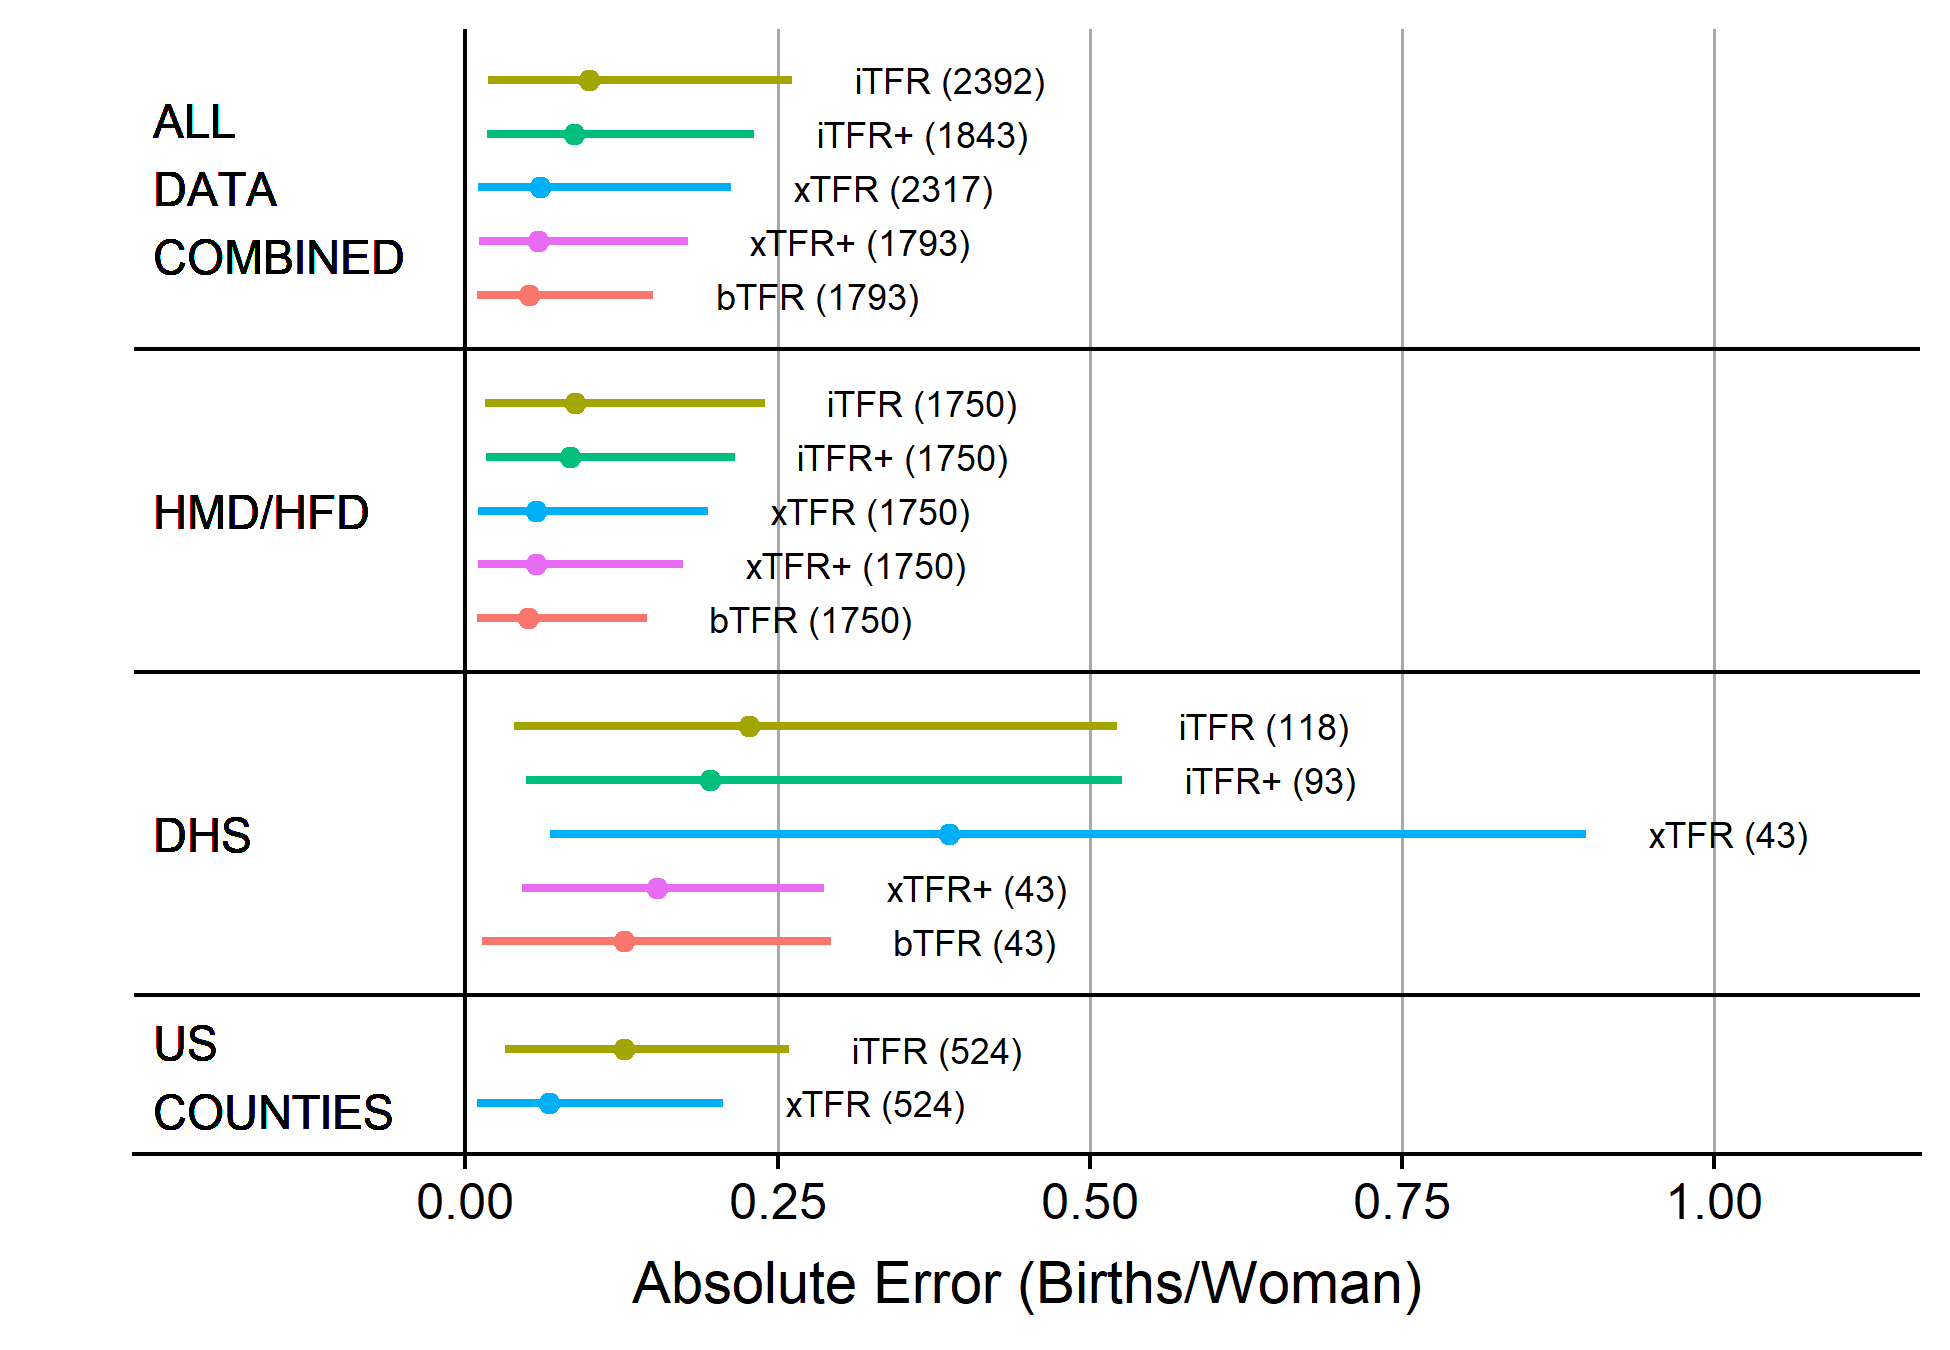
\includegraphics{manuscript_files/figure-latex/plot-comparisons-over-all-data-1.png}
\caption{\textbf{Absolute Error (Births/Woman) in TFR over alternative
methods and datasets.} Solid dots are at median Error for each method
and dataset. Horizontal bars extend from the 10th-90th percentile of
Error. Numbers in parentheses indicate the count of schedules for which
it is possible to use each method. Median errors are within 1/10th of a
birth across all data sets. \label{comparison}}
\end{figure}

\begin{figure}

{\centering 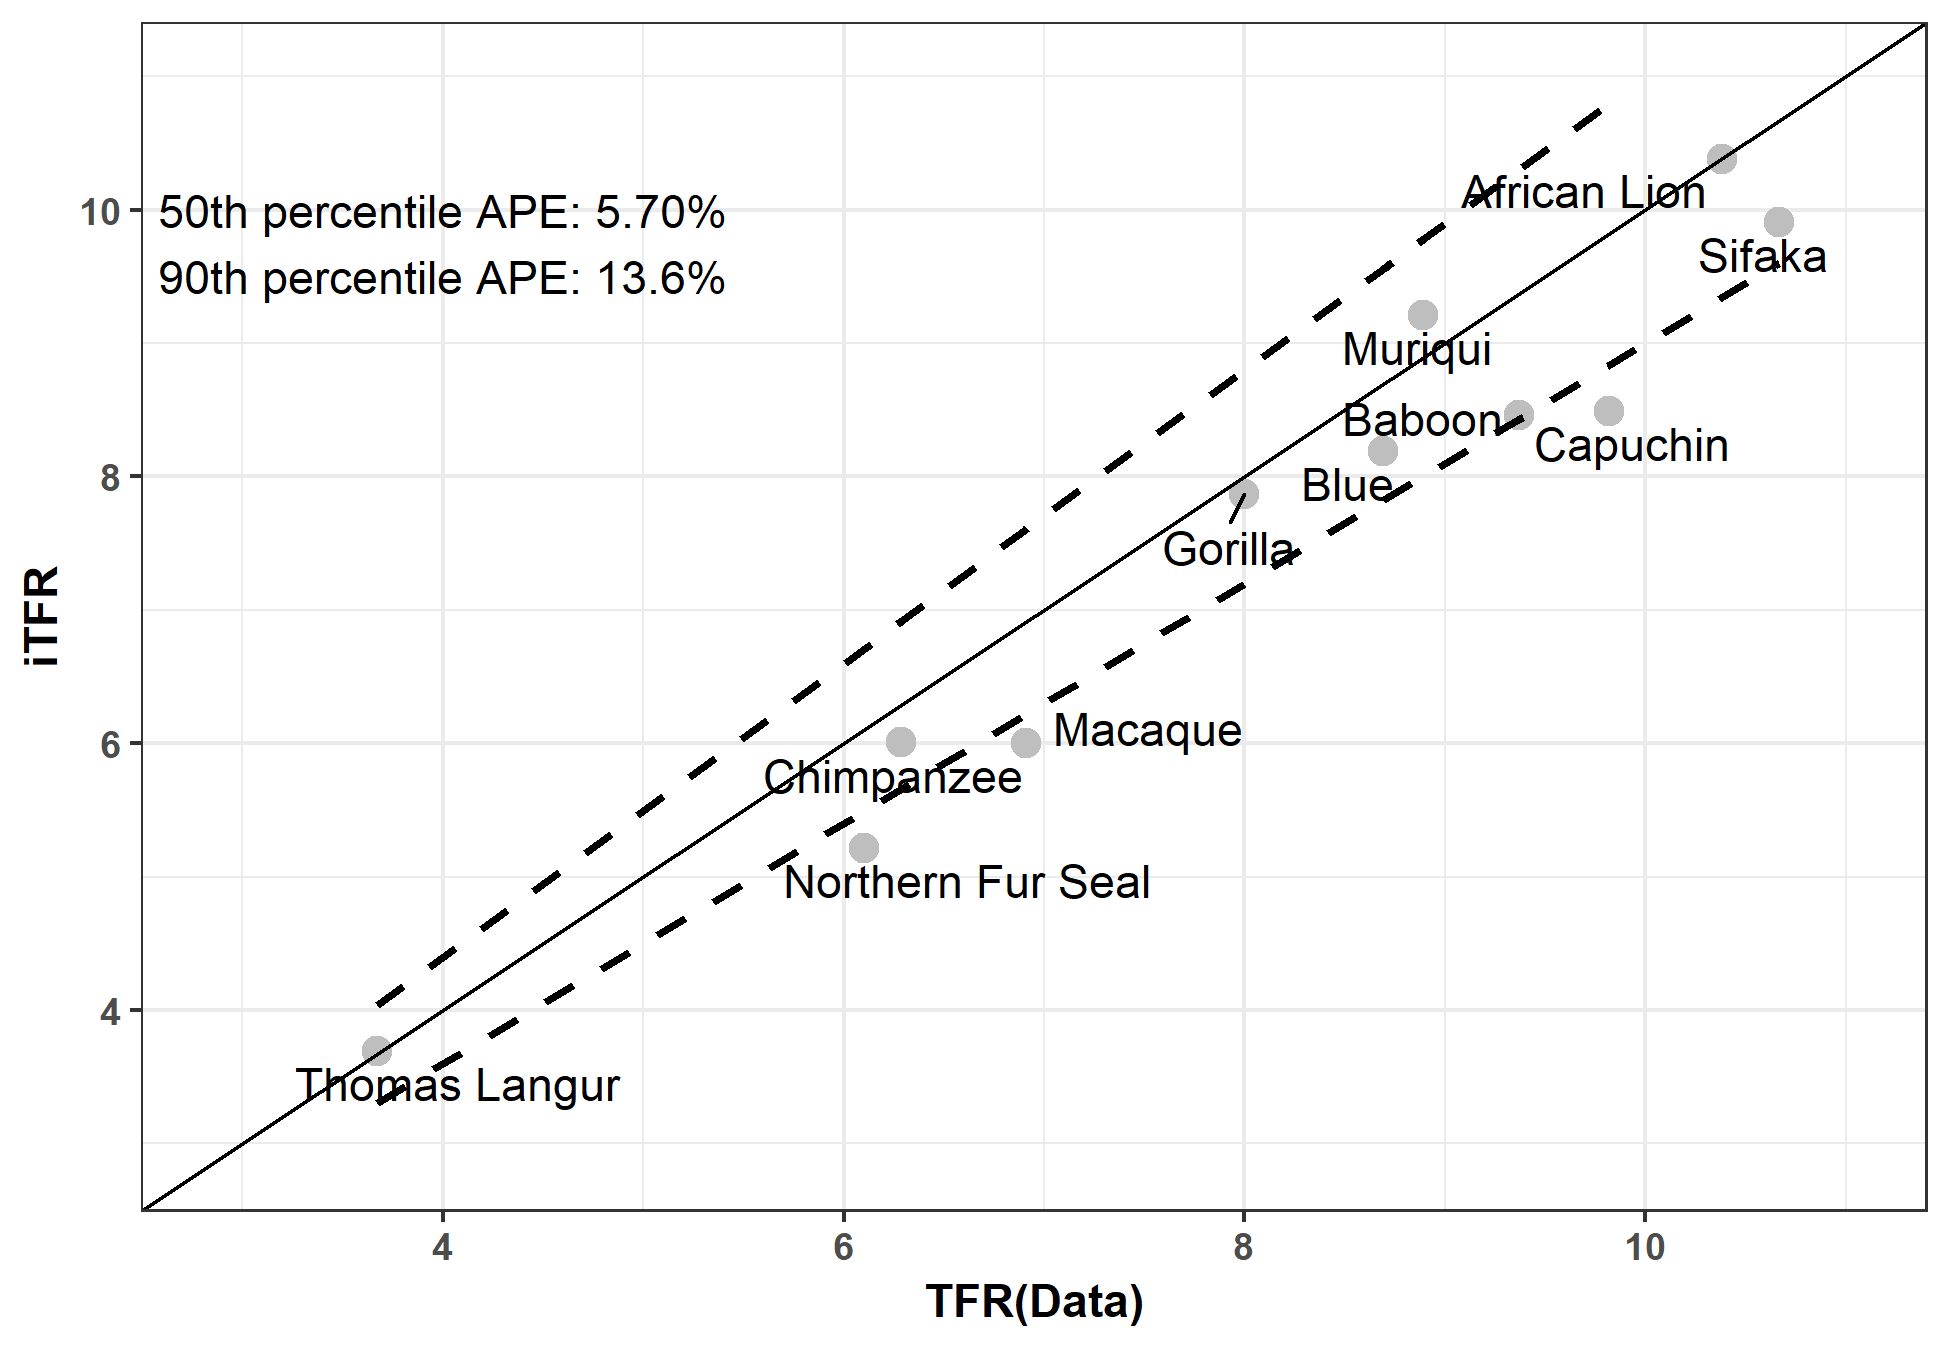
\includegraphics[width=0.6\linewidth]{manuscript_files/figure-latex/plot-nonhuman-estimates-1} 

}

\caption{\textbf{Fertility estimates for animal populations}. $iTFR$ estimates from nonhuman age-sex distributions. Observed TFR versus $iTFR$ estimates for the species listed in \autoref{nonhumantable}. Estimates match observations along the 45-degree line; dashed lines represent +/- 10\% errors.\label{primates}}\label{fig:plot-nonhuman-estimates}
\end{figure}

\hypertarget{errors-for-nonhuman-species}{%
\subsection{Errors for Nonhuman
Species}\label{errors-for-nonhuman-species}}

To test the generalizability of the method, we examine the accuracy of
the \(iTFR\) estimator in 11 nonhuman populations described in
(\textbf{\autoref{nonhumantable}}). We find that \(iTFR\) accurately
estimates total fertility among these species
(\textbf{\autoref{primates}}). These results suggest the method captures
fundamental properties that govern mammalian fertility, and that it
could be valuable in other studies with nonhuman populations.

\hypertarget{sensitivity-to-tfr-level-population-size-and-time-period}{%
\subsection{Sensitivity to TFR Level, Population Size, and Time
Period}\label{sensitivity-to-tfr-level-population-size-and-time-period}}

\begin{figure}
\centering
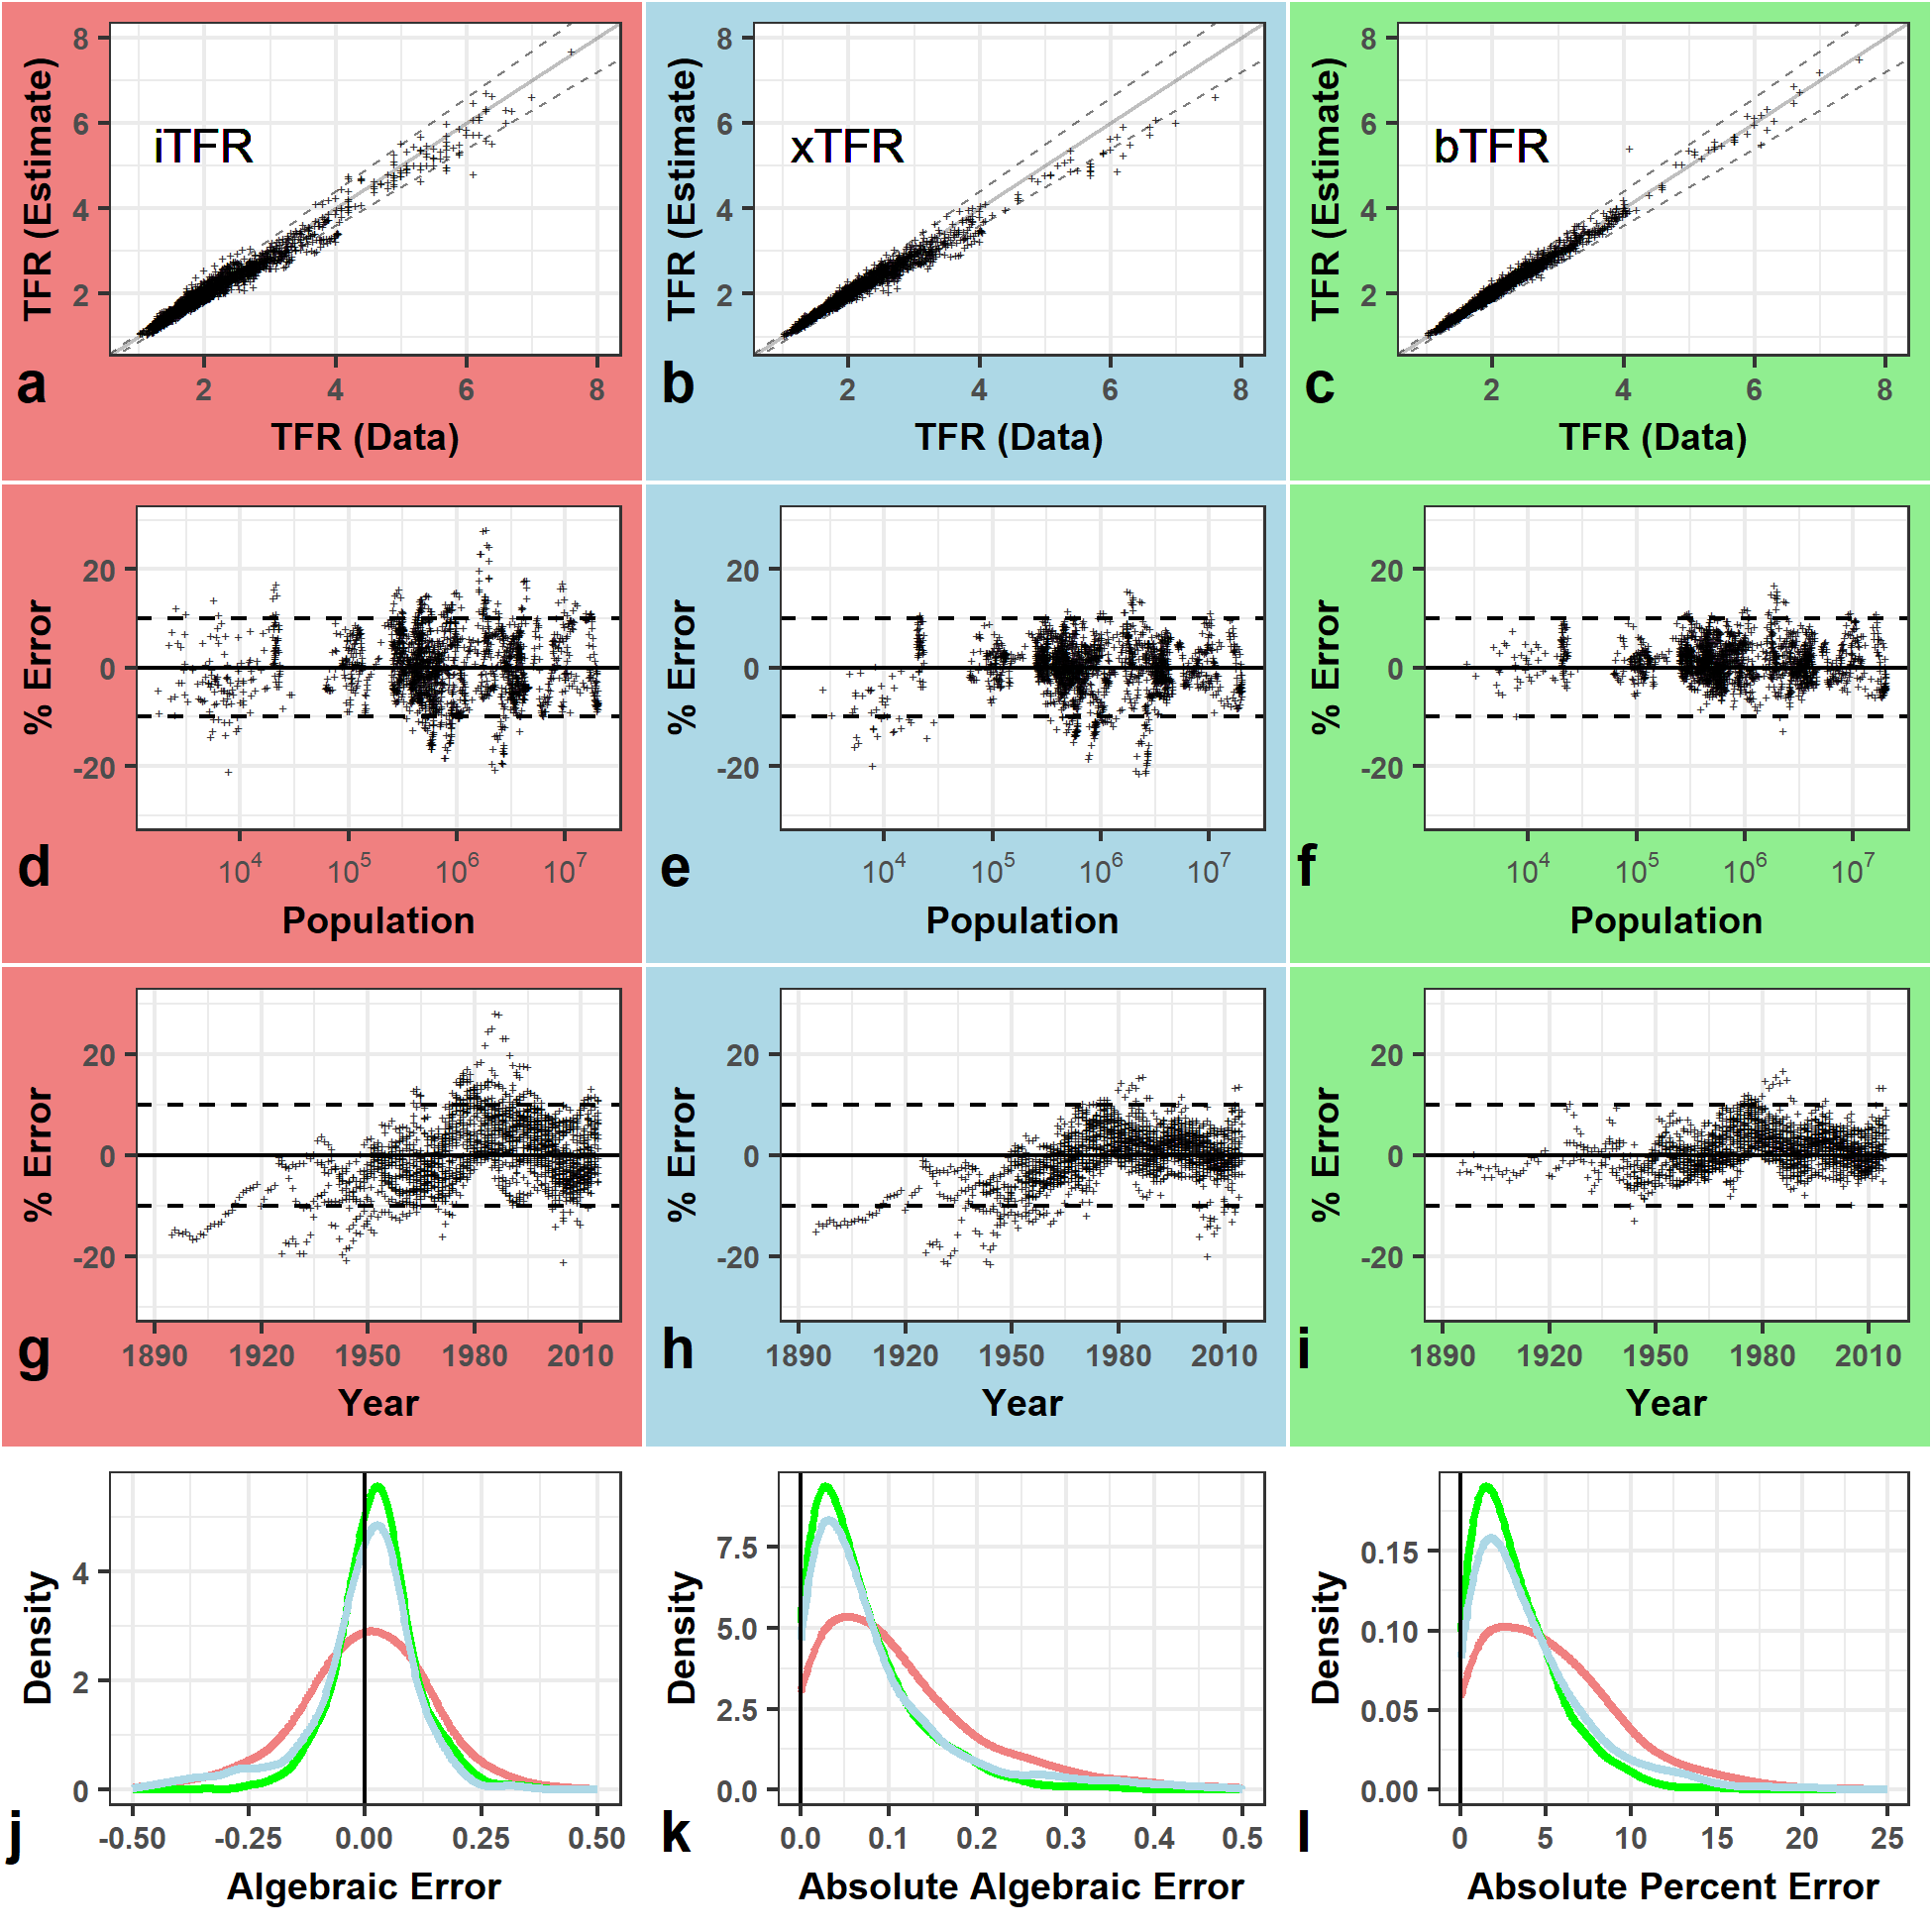
\includegraphics{manuscript_files/figure-latex/plot-multipanel-summary-1.png}
\caption{\textbf{Estimated TFR from Population Pyramids.} Performance of
three variants in HFD and DHS data. (a, d, g) use \(iTFR\); (b, e, h)
use \(xTFR\); (c, f, i) use \(bTFR\); (a, b, c) plot estimated TFR
against the observed 5-year average TFR. The solid line is \(Y=X\), and
the dashed lines are \(\pm 10\%\). (d, e, f) illustrate percent error
against population size. The dashed lines represent errors of
\(\pm 10\%\). (g, h, i) plot percent errors against the year in which
the population pyramid is observed. (j) plots the distribution of
algebraic errors for each method (\(est-obs\)). (k) plots the
distribution of absolute algebraic errors. (l) plots the distribution of
absolute percent errors. For all variants, estimates are accurate over
many scales and times. \label{multipanel-summary}}
\end{figure}

\textbf{\autoref{multipanel-summary}} reports the accuracy of \(iTFR\),
\(xTFR\), and \(bTFR\) estimators for the HFD/HMD and DHS data combined
for different levels of TFR, different population sizes, and different
historical periods. \textbf{\autoref{error-table}} reports summary
measures of the accuracy for all five estimators using the same combined
HFD/HMD and DHS data as well as U.S. counties. Overall, we find good
agreement between estimated and observed TFRs for all five estimators
(\textbf{\autoref{multipanel-summary}}, a, b, c and
\textbf{\autoref{error-table}}.

Demographic estimators are typically more accurate for larger
populations (due to the law of large numbers) and for more recent time
periods (due to improved data collection practices). However, we find
that error rates are independent of population size
(\textbf{\autoref{multipanel-summary}}, d, e, f) and are fairly stable
across time (\textbf{\autoref{multipanel-summary}}, g, h, i), suggesting
scale and temporal independence uncommon in other indirect methods.

Even the simplest and least accurate of the five variants, \(iTFR\),
predicts the total fertility rate with absolute errors of less than 0.09
births/woman in half of the HFD and DHS populations, and less than 0.26
births/woman in 90\% of the populations
(\textbf{\autoref{error-table}}). Absolute percent errors for \(iTFR\)
are also quite small relative to most indirect demographic estimators:
50\% of errors are within \(4.6\)\% of the true TFR, and 90\% are within
\(10.8\)\%. As shown in \textbf{\autoref{multipanel-summary}} and
\textbf{\autoref{error-table}}, the additional information contained in
the \(xTFR\) and \(bTFR\) estimators produce even smaller errors. In
short, we find that for national populations in countries with accurate
data and (mostly) low mortality, accurate \(TFR\) estimates from
population pyramids are possible.

\begin{table}[t]

\caption{\label{tab:unnamed-chunk-2}\label{error-table}\textbf{Summary statistics for the five variants using data from the HMD/HFD and DHS and U.S. counties.} APE is the Absolute Percent Error.}
\centering
\resizebox{\linewidth}{!}{
\begin{tabular}{llrllll}
\toprule
Data & Method Family & n & 50\%ile Absolute Error & 90\%ile Absolute Error & 50\%ile APE & 90\%ile APE\\
\midrule
 & iTFR & 118 & 0.23 & 0.52 & 4.7\% & 10.5\%\\

 & iTFR+ & 93 & 0.20 & 0.53 & 4.0\% & 11.1\%\\

 & xTFR & 43 & 0.39 & 0.90 & 8.4\% & 14.0\%\\

 & xTFR+ & 43 & 0.15 & 0.29 & 2.7\% & 6.6\%\\

\multirow{-5}{*}{\raggedright\arraybackslash DHS} & bTFR & 43 & 0.13 & 0.29 & 2.3\% & 5.3\%\\
\cmidrule{1-7}
 & iTFR & 1750 & 0.09 & 0.24 & 4.6\% & 10.7\%\\

 & iTFR+ & 1750 & 0.08 & 0.22 & 4.4\% & 10.3\%\\

 & xTFR & 1750 & 0.06 & 0.19 & 3.0\% & 8.2\%\\

 & xTFR+ & 1750 & 0.06 & 0.17 & 2.9\% & 7.4\%\\

\multirow{-5}{*}{\raggedright\arraybackslash HMD/HFD} & bTFR & 1750 & 0.05 & 0.15 & 2.6\% & 6.6\%\\
\cmidrule{1-7}
 & iTFR & 524 & 0.13 & 0.26 & 6.5\% & 12.8\%\\

\multirow{-2}{*}{\raggedright\arraybackslash US counties} & xTFR & 524 & 0.07 & 0.21 & 3.3\% & 10.1\%\\
\bottomrule
\end{tabular}}
\end{table}

\hypertarget{errors-in-subnational-estimates}{%
\subsection{Errors in Subnational
Estimates}\label{errors-in-subnational-estimates}}

It is possible that coefficients derived at the National level could
prove ineffective in estimating fertility at the subnational level (eg.
\citet{tuchfeld74}). \textbf{\autoref{error-table}} reports the errors
associated with both the \(iTFR\) and \(xTFR\) methods for U.S. counties
that also have corresponding observed total fertility rates. These
errors are on par with the errors observed using the HMD/HFD data,
demonstrating important consistency in low error rates across a variety
of scales.

\hypertarget{sensitivity-to-child-mortality}{%
\subsection{Sensitivity to Child
Mortality}\label{sensitivity-to-child-mortality}}

\begin{figure}
\centering
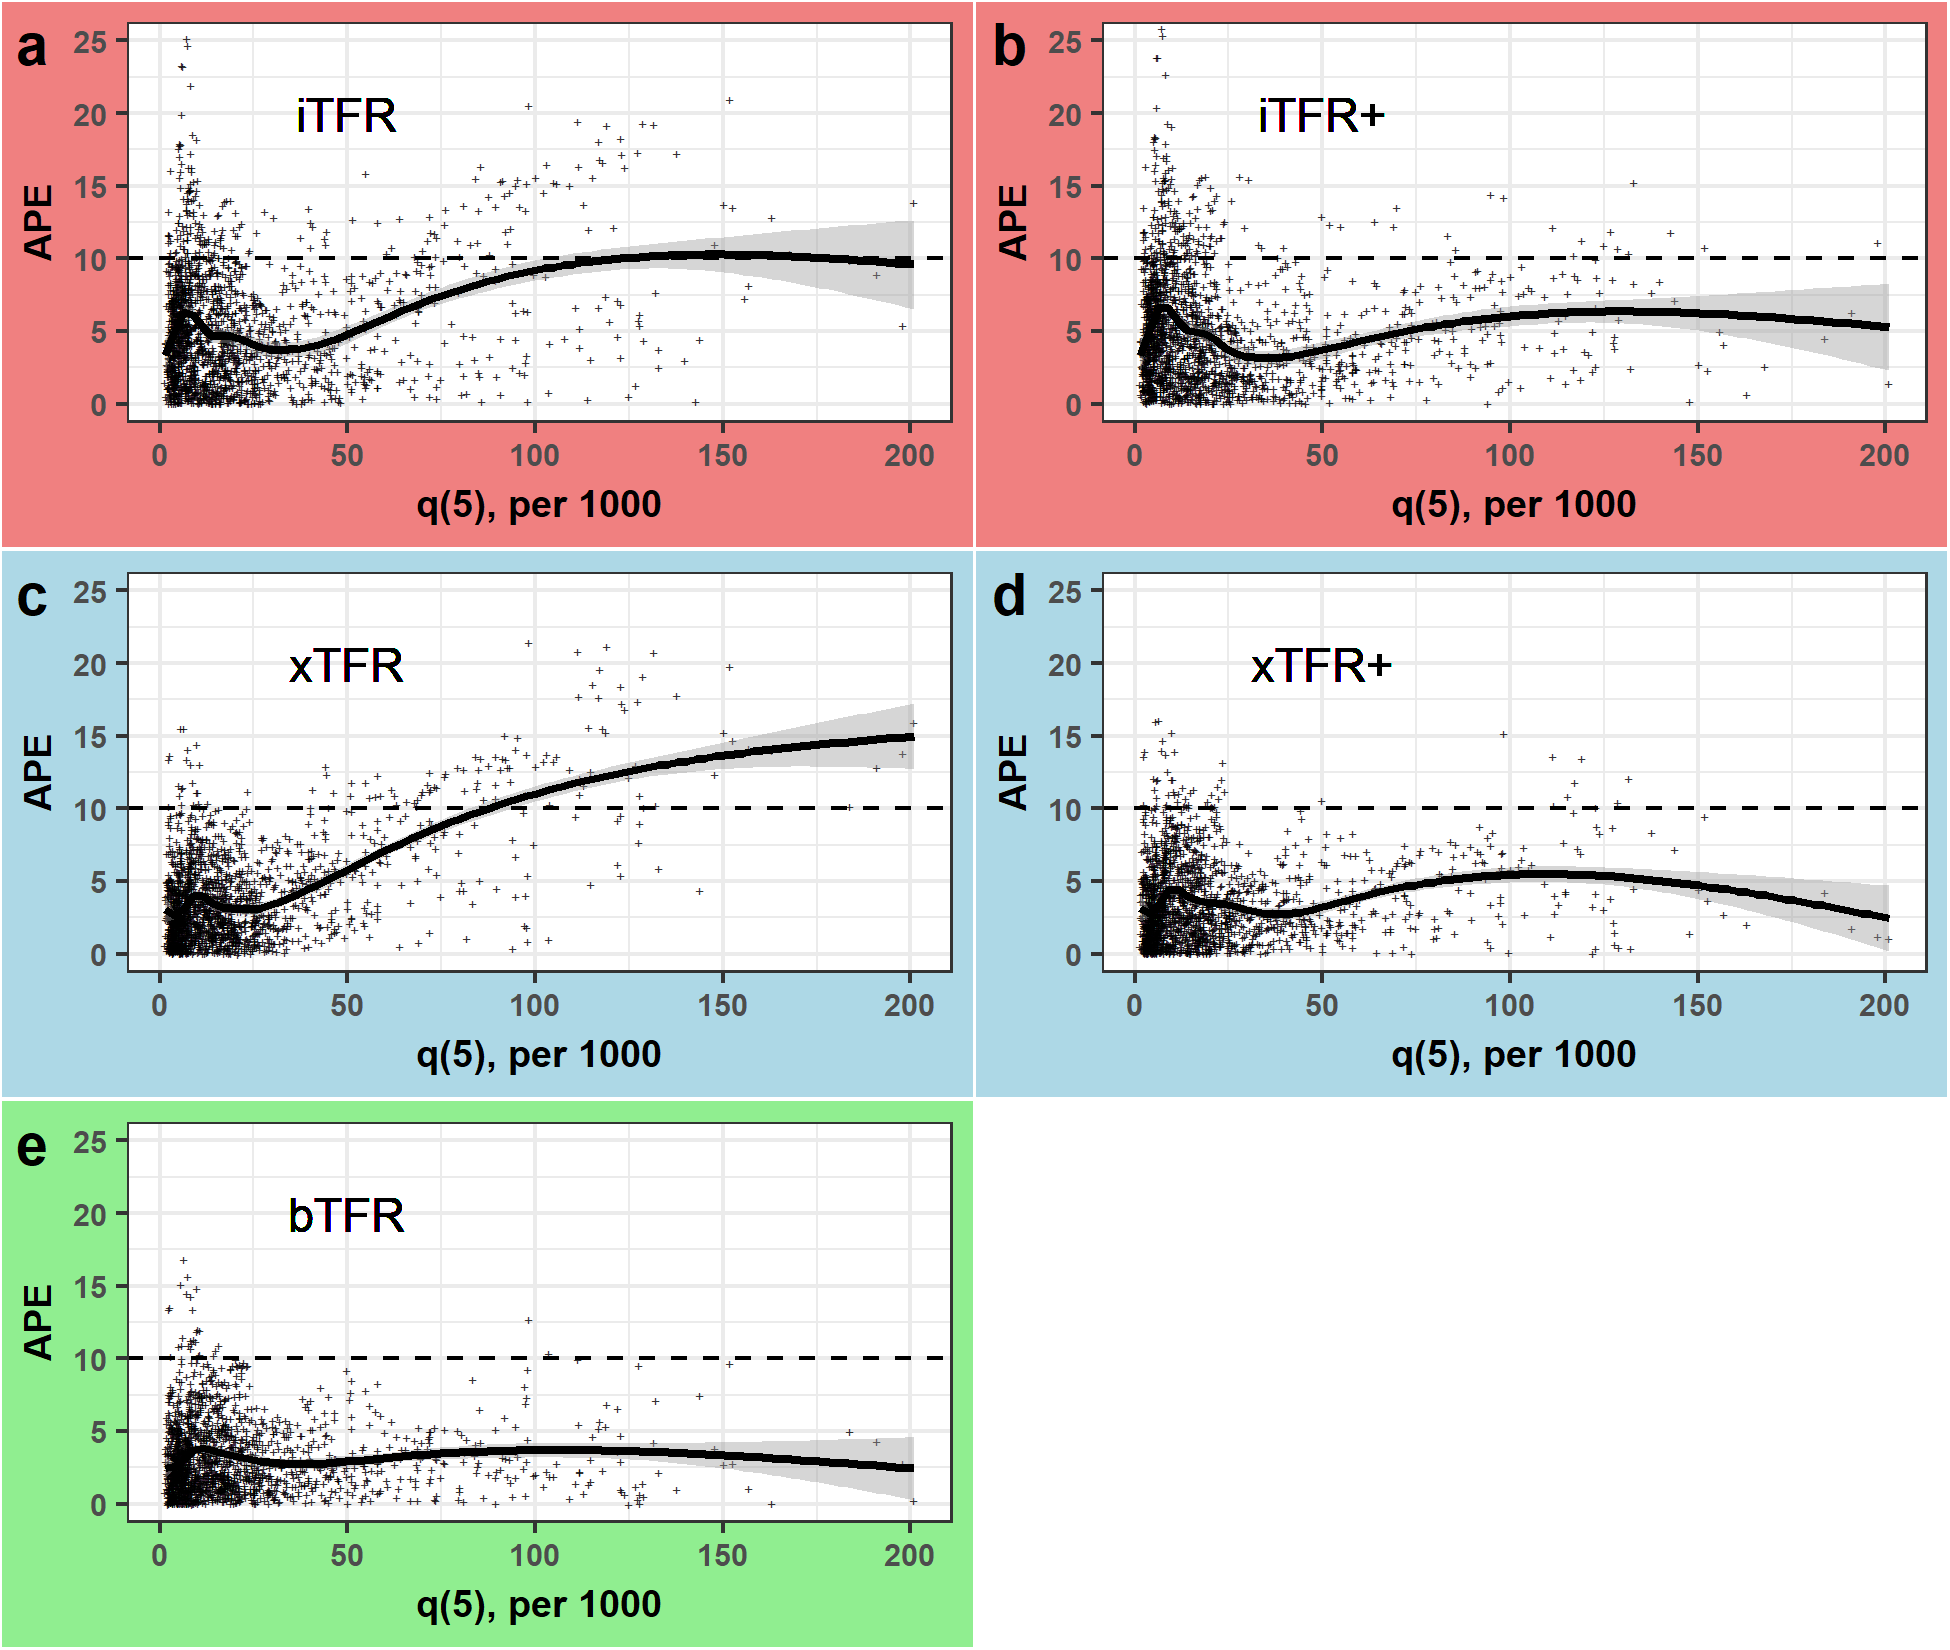
\includegraphics{manuscript_files/figure-latex/plot-errors-by-q5-1.png}
\caption{\textbf{Absolute Percent Errors against \(q_5\) values in the
HMD and DHS.} We compare the performance of the five variants against
observed \(q_5\) mortality rates. As \(q_5\) values increase, APE also
increases in the \(iTFR\) and \(xTFR\) variants. This is corrected in
the \(iTFR^+\), \(xTFR^+\), and \(bTFR\) variants, which incorporate
estimated child mortality. \label{errors-by-q5}}
\end{figure}

Our derivations for the \(iTFR\) and \(xTFR\) assume that child
mortality is negligible, and those estimators are likely to
underestimate fertility when it is not. We show this relationship in
\textbf{\autoref{errors-by-q5}} using data from the HMD/HFD and DHS,
where \(iTFR\) and \(xTFR\) produce increasing errors as child mortality
increases. Notice that the \(iTFR^+\), \(xTFR^+\), and \(bTFR\) variants
largely correct for higher mortality levels. Thus, in countries or
periods with high infant and child mortality, the \(iTFR^+\),
\(xTFR^+\), and \(bTFR\) variants are more appropriate.

\hypertarget{sec:extensions}{%
\subsection{Extensions}\label{sec:extensions}}

Accurate estimation of \(TFR\) from age-sex pyramids greatly expands our
ability to estimate fertility across varying geographies, time periods,
and subpopulations. To demonstrate the flexibility of the method, we
produce TFR estimates for three cases in which direct \(TFR\) estimation
is impossible.

\emph{Subnational Fertility in Africa}

We use data from WorldPop's gridded population age-structure data for
the year 2015 \citep{tatem2013millennium} in conjunction with \(q_5\)
estimates from the United Nations World Population Prospects 2017
\citep{united2017world} to produce subnational estimates of \(iTFR^+\)
for Africa. Scholars have increasingly published subnational estimates
of demographic indicators to monitor progress towards the UN's
Sustainable Development Goals (SDGs)
\citep{osgood2018mapping, golding2017mapping, graetz2018mapping} and our
framework allows a nearly unprecedented level of geographic detail
regarding fertility (\textbf{\autoref{WorldPop}}).

\begin{figure}
\centering
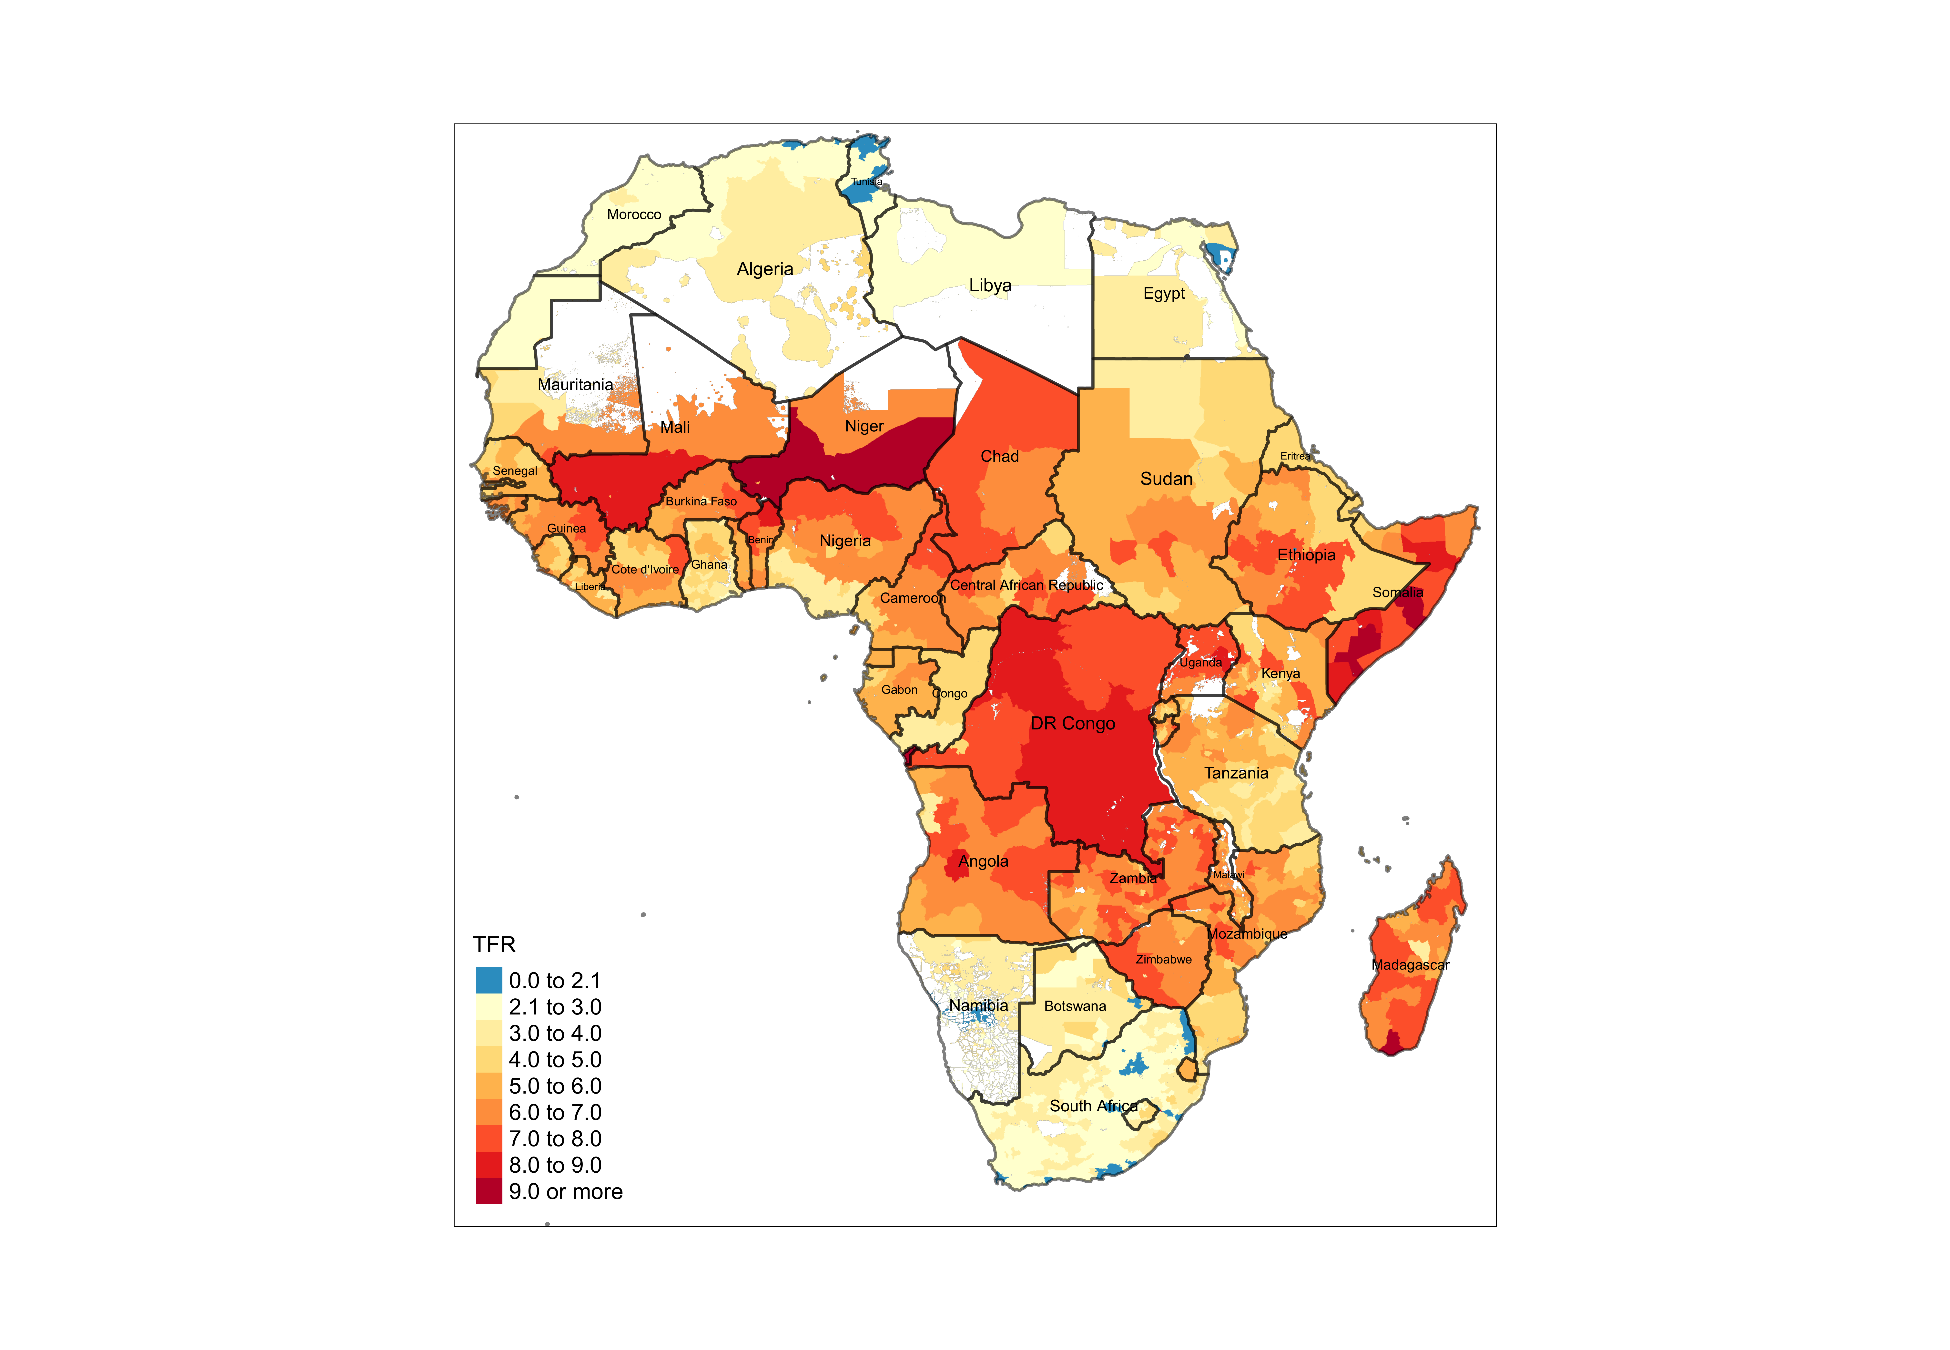
\includegraphics{manuscript_files/figure-latex/plot-africa-map-1.png}
\caption{\textbf{Estimating subnational fertility rates.} We use the
\(iTFR^+\) method to estimate subnational total fertility rates for the
African continent for 2010-2015 using data from WorldPop and the United
Nations WPP 2017. \label{WorldPop}}
\end{figure}

\emph{Historical Fertility in Europe}

We also extend our analysis of the Human Mortality Database by producing
fertility estimates for all 2955 country-years of data in the HMD (an
additional 1000 country-years' of estimates prior to the collection of
detailed birth records). From this large historic volume of data, we
highlight our findings in four example countries: France, Italy, the
Netherlands, and Sweden (\textbf{\autoref{Historic}}). Sweden began
tabulating the detailed birth records necessary for \(TFR\) calculation
in 1891, France in 1946, the Netherlands 1950, and Italy in 1954.
However, these countries collected both mortality and age-sex data
considerably earlier (1751 for Sweden, 1816 for France, 1850 for the
Netherlands, and 1872 for Italy). By using the \(bTFR\) method, we can
reconstruct historical TFRs to create a time series of fertility data
well before age-specific birth collection began, significantly expanding
our ability to explore historical fertility patterns from up to 250
years ago.

\begin{figure}
\centering
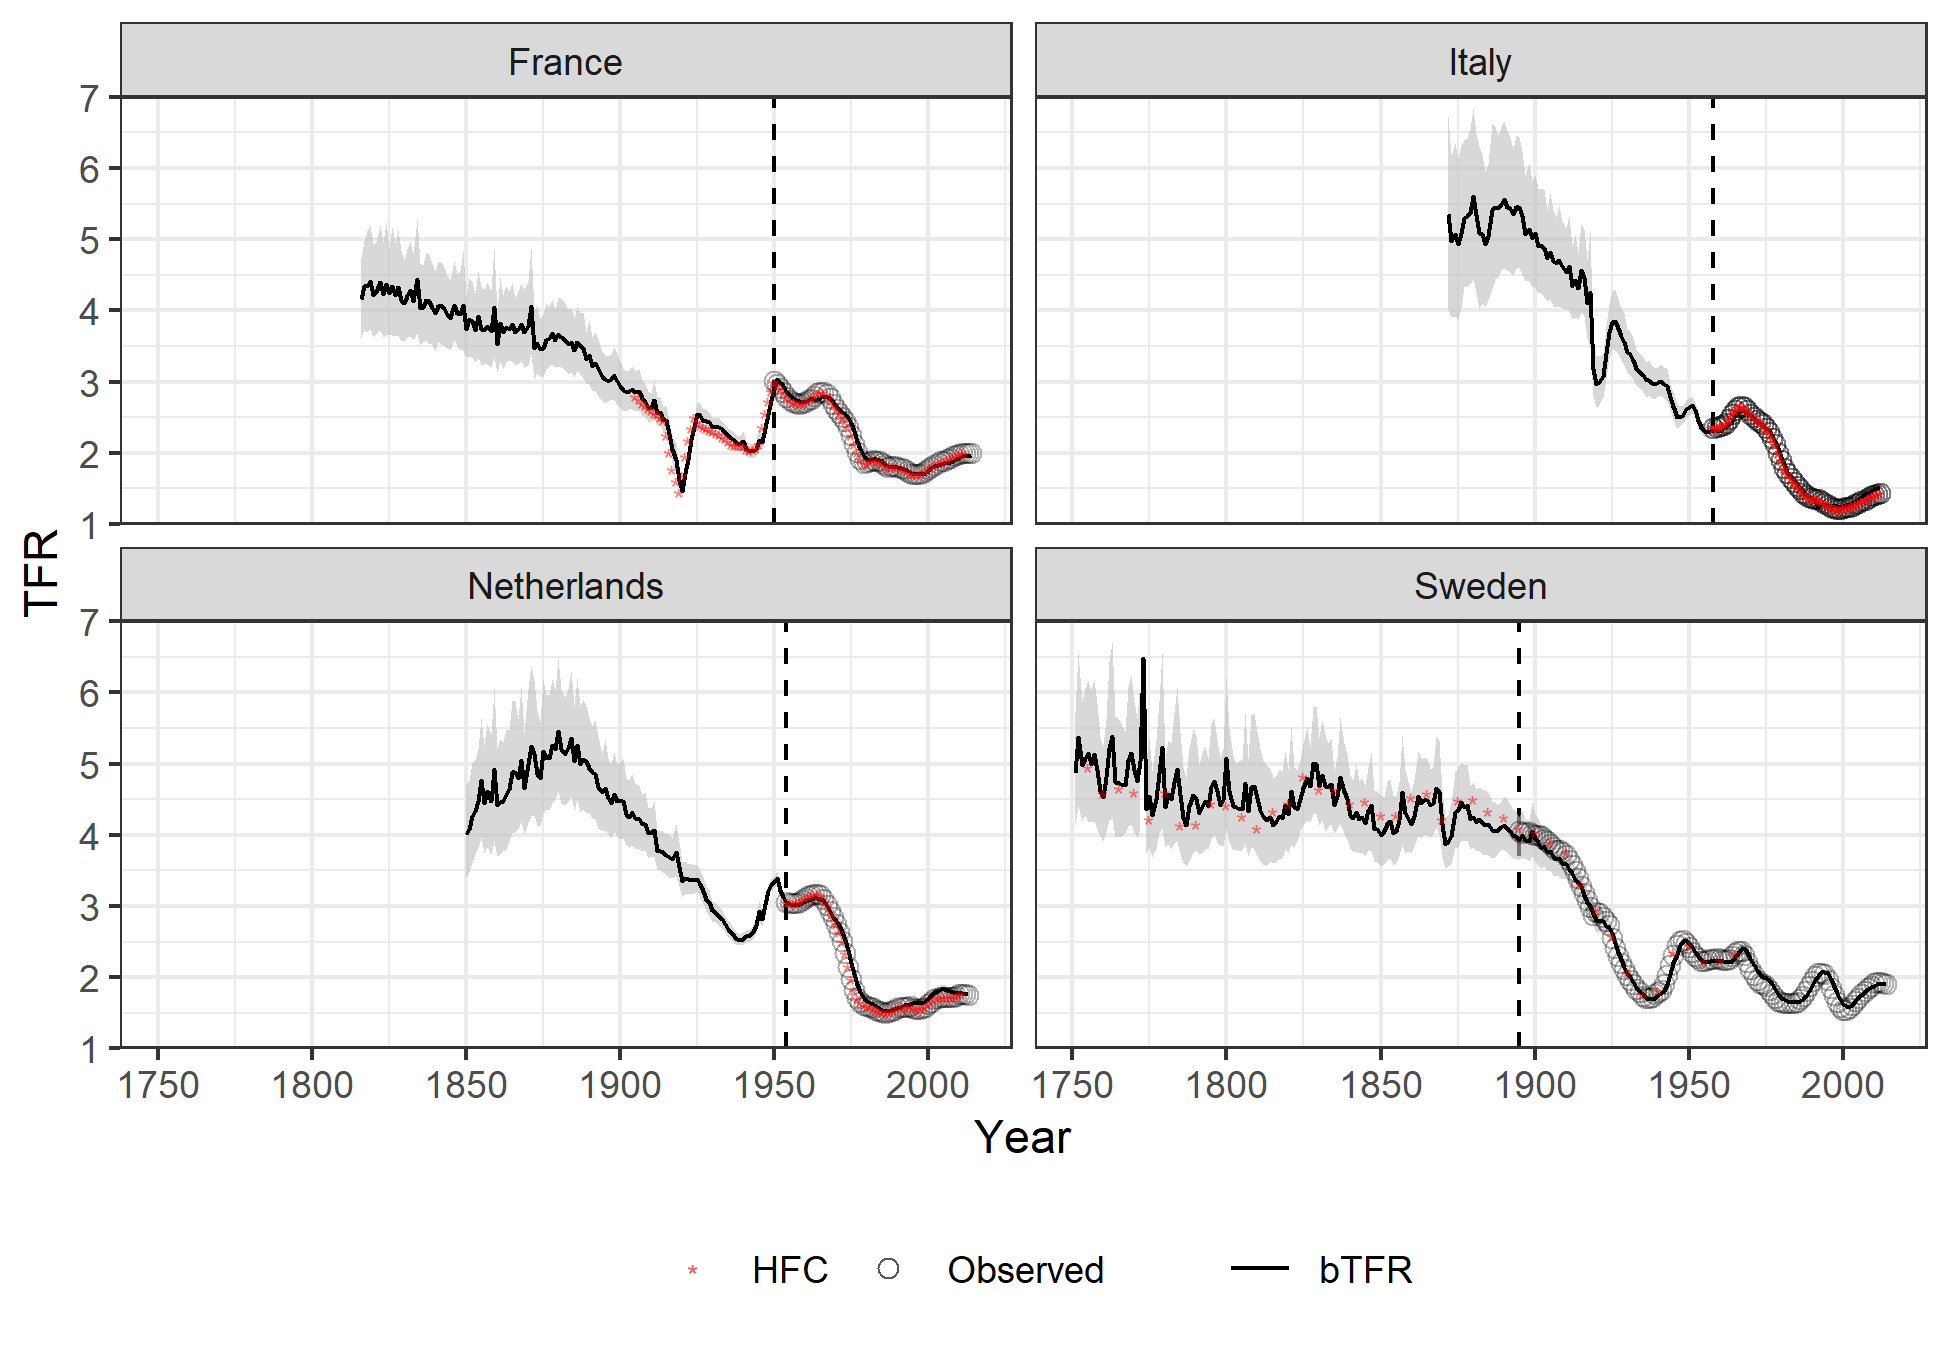
\includegraphics{manuscript_files/figure-latex/plot-historical-hmd-estimates-1.png}
\caption{\textbf{Estimating historical fertility.} \(bTFR\) estimates of
period fertility rates in four European countries using HMD historical
age-sex and child mortality data. Shaded regions represent 90 percent
posterior probability intervals; open circles are observed TFRs from the
HFD. Red stars are average TFRs over the preceding five-year period for
the earliest series with a vital records source from the Human Fertility
Collection \citep{HFC}.\label{Historic}}
\end{figure}

\emph{Fertility by Income and Race in the United States}

The complex connections between fertility and household income have
always interested demographers
\citep{becker1960economic, jones2008fertility}. However, analysis is
limited because birth certificates do not include economic information,
and very few surveys include both income and fertility questions.
Estimation of fertility levels from population composition can expand
our ability to learn about fertility-income correlations in different
social groups.

(\textbf{\autoref{Income}}) provides an example. We use the \(xTFR\)
method to estimate TFRs conditional on both race (White/Non-White) and
household income level in the United States, using data on the age-sex
composition of households in different income strata from the Current
Population Survey (CPS). Data for this figure comes from aggregated
2010--2018 March Economic Supplements, downloaded from IPUMS
\citep{IPUMSCPS}. Indirect methods based on age-sex data allow us to
produce estimates of \(TFR\) by income groups, and to further
disaggregate by race. Among both Whites and Non-Whites, there is a
definite U-shaped relationship, with the highest fertility levels in the
poorest and richest American households.

Here we provide these examples only as a proof of concept: indirect
fertility estimation identifies intriguing relationships that would not
be estimable by other means, and which clearly merit further study.

\begin{figure}
\centering
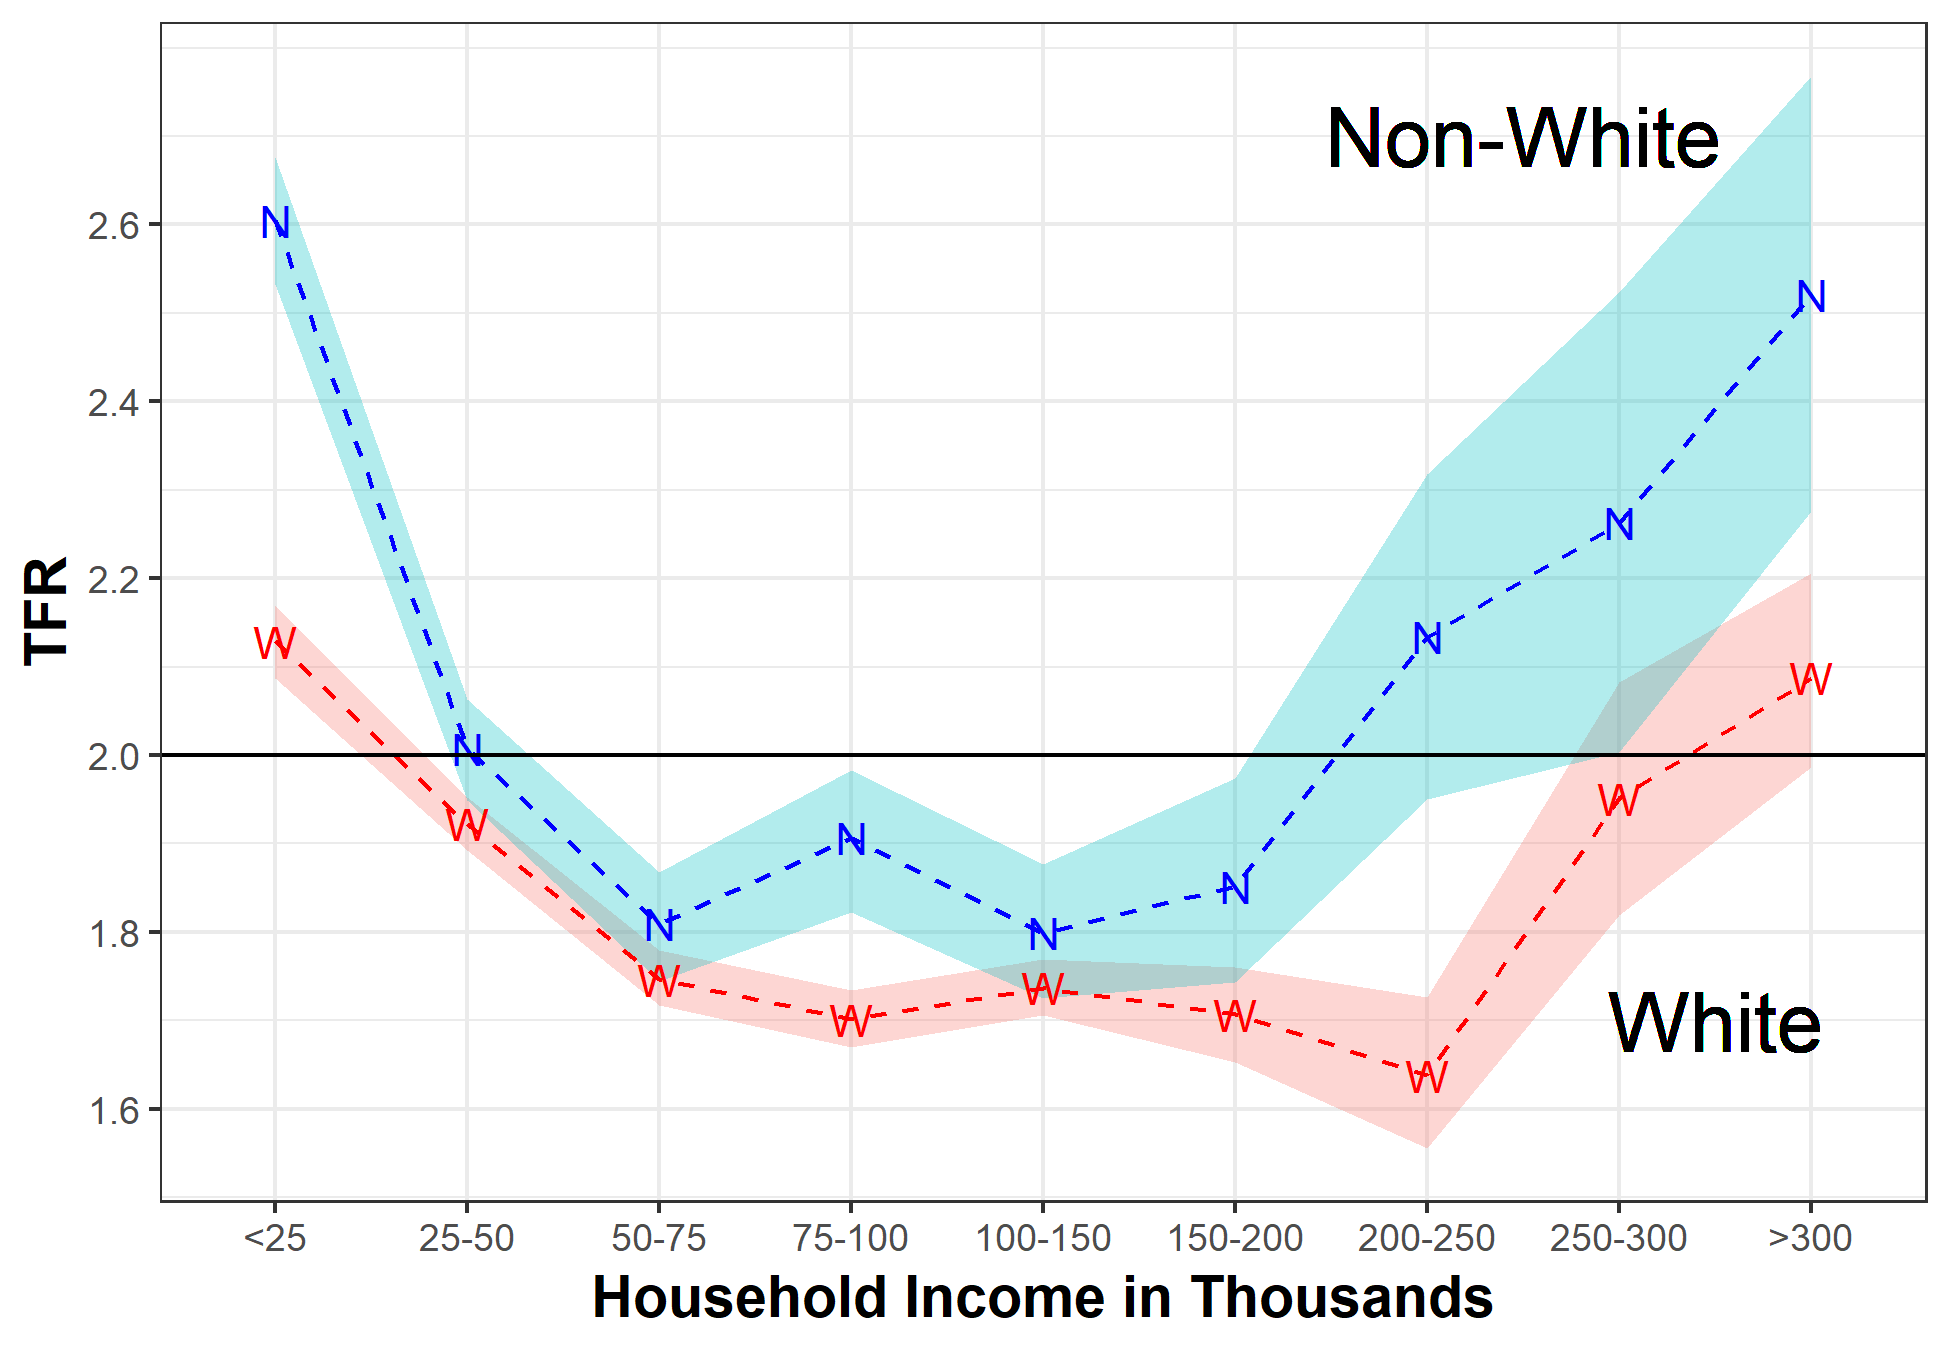
\includegraphics{manuscript_files/figure-latex/resample-CPS-income-race-1.png}
\caption{\textbf{Total Fertility (\(xTFR\)) by race and household income
level.} We estimate TFR from age-sex distributions within race-income
categories using the U.S. Current Population Survey (CPS) March Social
and Economic Supplements, combined over 2010-2018. White corresponds to
those reporting their race as White only; Non-White corresponds to all
other survey respondents. Shaded regions represent confidence intervals
(5\%-95\%) estimated from 1000 bootstrap samples in which households in
each rae-income category are drawn randomly with replacement from the
set of all CPS households. \label{Income}}
\end{figure}

\hypertarget{conclusion}{%
\section{Conclusion}\label{conclusion}}

We have examined our framework's errors using high-quality age pyramids
and fertility data. With a few minor caveats, we conclude that indirect
estimators yield accurate \(TFR\) estimates when age-sex input data is
accurate.

Researchers should use caution, however, when applying our framework in
data environments with potentially deficient inputs. The methods
outlined above produce good estimates of \(TFR\), but they require
accurate age-sex counts. Underenumeration of children aged 0-4 is a
well-known problem with census data
\citep{ewbank1981age, o2014historical, o2015coverage}, and misreporting
of children aged 0-4 will yield inaccurate estimates of total fertility
in our framework. Future extensions could adjust for underenumeration,
either by adding an undercount multiplier to Equation (\ref{eq:s0TFR}),
or by including a prior distribution for undercount in the \(bTFR\)
model.

Demographers should use expert judgement when choosing which variant to
employ. For instance, in populations with known or suspected high child
mortality one should likely estimate \(TFR\) using \(iTFR^+\),
\(xTFR^+\), or \(bTFR\) to correct for child mortality (if \(q_5\)
estimates are available). In choosing the three example extensions in
\autoref{sec:extensions}, we chose the variant to fit both the data
available and known demographic characteristics of the population. We
know Africa tends to have high child mortality but we are also cautious
about the accuracy of WorldPop's age-structure data. This led us to
\(iTFR^+\), which corrects for child mortality but does not use the
detailed age distribution for women of childbearing ages. Similarly, the
HMD contains high quality data but the further back in time one goes the
more important uncertainty about child mortality becomes. In this
situation \(bTFR\) is the appropriate method. To estimate U.S. fertility
conditional on household income and race, we do not have child mortality
available for these populations. However, U.S. child mortality is quite
low, and for small subpopulations the age structure among
reproductive-age women is quite variable. These considerations make
\(xTFR\) the most appropriate estimator. Scholars should use similar
judgements when using our framework to answer their own research
questions.

Our framework's flexible data requirements allow researchers to select
the variant that conforms to the available data, and offers high
confidence for estimates. As we show in our example extensions, this
approach opens the door to fertility analyses for many populations of
interest to sociologists \citep{lesthaeghe14}, economists
\citep{hotz1997economics}, anthropologists
\citep{greenhalgh1995situating}, epidemiologists
\citep{paulson2002pregnancy}, historians \citep{woods2000demography},
and population geographers \citep{sorichetta2015high}.

There is now increased demand for high-resolution gridded population
datasets for climate change research and SDGs
\citep{jones15, cincotta00, golding2017mapping}. Because our methods
work well for small populations, scientists could use them to estimate
small-area fertility levels and changes, as inputs to gridded population
projections or for gridded fertility level datasets.

Because they rely on basic, commonly collected census data the
parameter-free, scale-, time-, and species-robust techniques can
estimate total fertility even in areas without detailed demographic
data. We anticipate this estimation framework will open new lines of
inquiry into human fertility patterns.

\hypertarget{replication-files}{%
\section{Replication Files}\label{replication-files}}

All data and code necessary to reproduce the reported results are
licensed under the CC-BY-4.0 license and are publicly available in a
replication repository located at
(\url{https://github.com/mathewhauer/iTFR-replication}). The analyses
were performed in \emph{R} \citep{rcite}. For the \(bTFR\) variant we
use the \emph{rstan} package \citep{rstanpackage} to inferface with Stan
\citep{stanjss2017}.

\newpage

\hypertarget{supplementary-material}{%
\section*{Supplementary material}\label{supplementary-material}}
\addcontentsline{toc}{section}{Supplementary material}

\setcounter{table}{0} \renewcommand{\thetable}{S\arabic{table}}\setcounter{figure}{0} \renewcommand{\thefigure}{S\arabic{figure}}

\begin{table}[H]

\caption{\label{tab:make-table-hfd-countries}\label{HFDCountries}\textbf{Human Fertility Database Countries and years of data availability.}}
\centering
\begin{tabular}{llll}
\toprule
Country & Data Avail. (\# of Years) & Country & Data Avail. (\# of Years)\\
\midrule
Austria & 1951-2014 (64) & Iceland & 1960-2012 (53)\\
Bulgaria & 1947-2009 (63) & Italy & 1954-2014 (61)\\
Belarus & 1964-2014 (51) & Japan & 1947-2014 (68)\\
Canada & 1921-2011 (91) & Lithuania & 1959-2014 (56)\\
Switzerland & 1932-2014 (83) & Netherlands & 1950-2014 (65)\\
\addlinespace
Chile & 1992-2005 (14) & Norway & 1967-2014 (48)\\
Czechia & 1950-2014 (65) & Poland & 1971-2014 (44)\\
Germany & 1956-2013 (58) & Portugal & 1940-2015 (76)\\
Spain & 1922-2014 (93) & Russia & 1959-2014 (56)\\
Estonia & 1959-2014 (56) & Slovakia & 1950-2009 (60)\\
\addlinespace
Finland & 1939-2015 (77) & Slovenia & 1983-2014 (32)\\
France & 1946-2015 (70) & Sweden & 1891-2014 (124)\\
Northern Ireland & 1974-2014 (41) & Taiwan & 1976-2014 (39)\\
Scotland & 1945-2014 (70) & Ukraine & 1959-2013 (55)\\
England and Wales & 1938-2014 (77) & USA & 1933-2015 (83)\\
\addlinespace
Hungary & 1950-2014 (65) &  & \\
\bottomrule
\end{tabular}
\end{table}

\newpage

\bibliographystyle{agsm}
\bibliography{mybibfile}

\end{document}
